\documentclass[a4paper,notitlepage,parskip=full]{scrreprt}

\title{Cluster Coffer Manual}
\author{
	Alexander Hirsch\\
	\href{mailto:alex@dps.uibk.ac.at}{\texttt{alex@dps.uibk.ac.at}}
	\and
	Daniel Gröber\\
	\href{mailto:daniel@dps.uibk.ac.at}{\texttt{daniel@dps.uibk.ac.at}}
}
\date{}

% font
\usepackage{microtype}
\usepackage[no-math]{fontspec}
	\setmainfont{TeX Gyre Termes}
	\setsansfont{TeX Gyre Heros}
	\setmonofont{Inconsolata}[Scale=0.9]
	\addtokomafont{disposition}{\rmfamily}

% page
% \usepackage[margin=1in,showframe]{geometry}
\usepackage[margin=1in]{geometry}

% colour
\usepackage{xcolor}
	\definecolor{linkcolor}{cmyk}{1.0, 0.6, 0.0, 0.56}

% links
\usepackage{hyperref}
	\hypersetup{
		colorlinks      = true,
		citecolor       = linkcolor,
		citebordercolor = linkcolor,
		linkcolor       = linkcolor,
		linkbordercolor = linkcolor!40,
		urlcolor        = linkcolor,
		pdfstartview    = {XYZ null null null},
		pdfpagemode     = UseOutlines,
	}
	\urlstyle{same}

% math
\usepackage{amsmath}

% references
\usepackage[capitalise,noabbrev]{cleveref}

% graphics
\usepackage{graphicx}
\usepackage{pdfpages}

% tables
\usepackage{longtable}
\usepackage{booktabs}

% misc
\usepackage{scrhack}

\begin{document}

\maketitle

The \textit{Cluster Coffer} is a portable, all-in-one HPC cluster designed for demonstration purposes.
Its design makes it ideal for cramped PR events.
Just place it on a level surface, plug it in, and you are ready to compute.

This document serves as a manual for assembly and maintenance.
Furthermore, similar projects can be bootstrapped from this.
Throughout the document, take note of the elegant, yet modular design.

It mainly consists of one head node, 16 compute nodes, a switch, and power distribution.

The first chapter is a step-by-step assembly guide.
Most steps require detailed information found in the following chapters.
It is recommended to read through this document from top to bottom before touching anything.

\tableofcontents

\chapter{Assembly}

This chapter covers the big-picture of assembling the system and depends heavily on the following ones.
A rudimentary bill of materials can be found in \cref{bom}.

\begin{itemize}
	\item First things first: assemble a sandwich for culinary motivation.
	\item Place the base-plate into the case and drill the ten mounting holes into the bottom of the case.
	\item Take the base-plate out, we'll come back to it later on.
	\item Install the mains power socket (with switch and fuse) into the back of the case.
	\item Replace the heatsink of the head node.
	\item Install the head node into the inside of the lid of the case.
	\item Put together the frame, double check the mounting nuts sizes, count, and location.
	\item Align the frame's M5 nuts with the corresponding holes in the base-plate and fix them in place using hot glue.
	\item Install both power supplies, the switch, and the power conduit box onto the base-plate.
	\item Connect the power supplies and the switch with the power conduit box.
	\item Add the cable used for connecting the power conduit box with the mains power socket.
		Only connect it to the conduit box for now.
	\item Connect the frame to the base-plate using six M4 screws (front, left, right).
	\item Eat the sandwich.
	\item Assemble the custom circuit boards.
	\item Put together the four panels holding 4 compute nodes each.
	\item Attach a 0.5 m network cable to the switch.
		This one is used for the head node.
	\item Attach a long network cable to the switch.
		This one can be used to connect the system to a network / computer.
	\item Attach the 12 V power cable for the head node to the 12 V power supply.
	\item Attach two 0.25 m network cables and two 0.5 m network cables to the switch.
	\item Place the last panel (nodes 13--16) upside down in front of the frame-base-plate assembly.
	\item Connect the 12 V fan power cable and the 5 V compute node power cable to the panel assembly.
	\item Mount the panel assembly to the frame, the two 0.25 m network cables go in front of the panel, the other two go behind.
		Push the panel all the way to the back before tightening the screws.
	\item Connect the four network cables to the panel assembly.
	\item Repeat for the remaining three panel assemblies.
	\item Connect the power conduit to the mains power socket with the cable you almost forgot about.
	\item Lower the frame-base-plate-panel assembly into the case.
	\item Connect the head node's power and network cable.
	\item Fasten the frame-base-plate-panel assembly through the bottom of the case using M5 screws.
	\item Connect all remaining cables.
	\item Grab your coffee mug, put on some safety glasses, and hit the power button.
	\item \textit{Explosion}
	\item \dots
	\item Profit!
\end{itemize}

\chapter{Metalware}

This chapter covers the mechanical part of the build.
Note that the construction requires access to a workshop as most parts are custom.

Software:

\begin{itemize}
	\item Autodesk Inventor Professional 2013
\end{itemize}

\section{Frame}

A frame consisting of 2020 aluminium extrusions serves as mechanical backbone for everything.
Other parts, like the base-plate, are connected to it.
In the final steps of the assembly, the frame is lowered into the case with all components attached and fastened to the case.

Navigate to the corresponding section in \cref{bom}.

Assembling the frame is straight forward.
Just watch out to insert the correct nuts into the correct grooves:

\begin{center}
	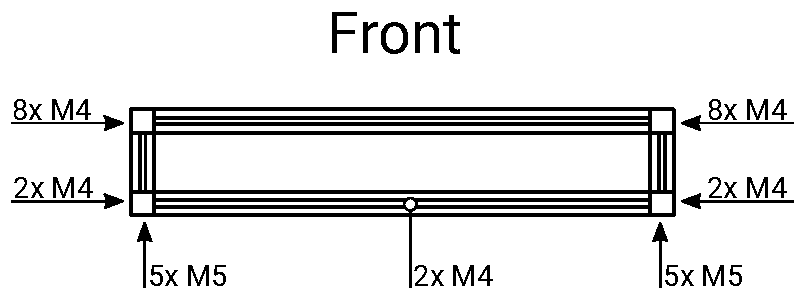
\includegraphics[width=0.95\textwidth]{inc/drawing_frame_front_nuts.pdf}
\end{center}

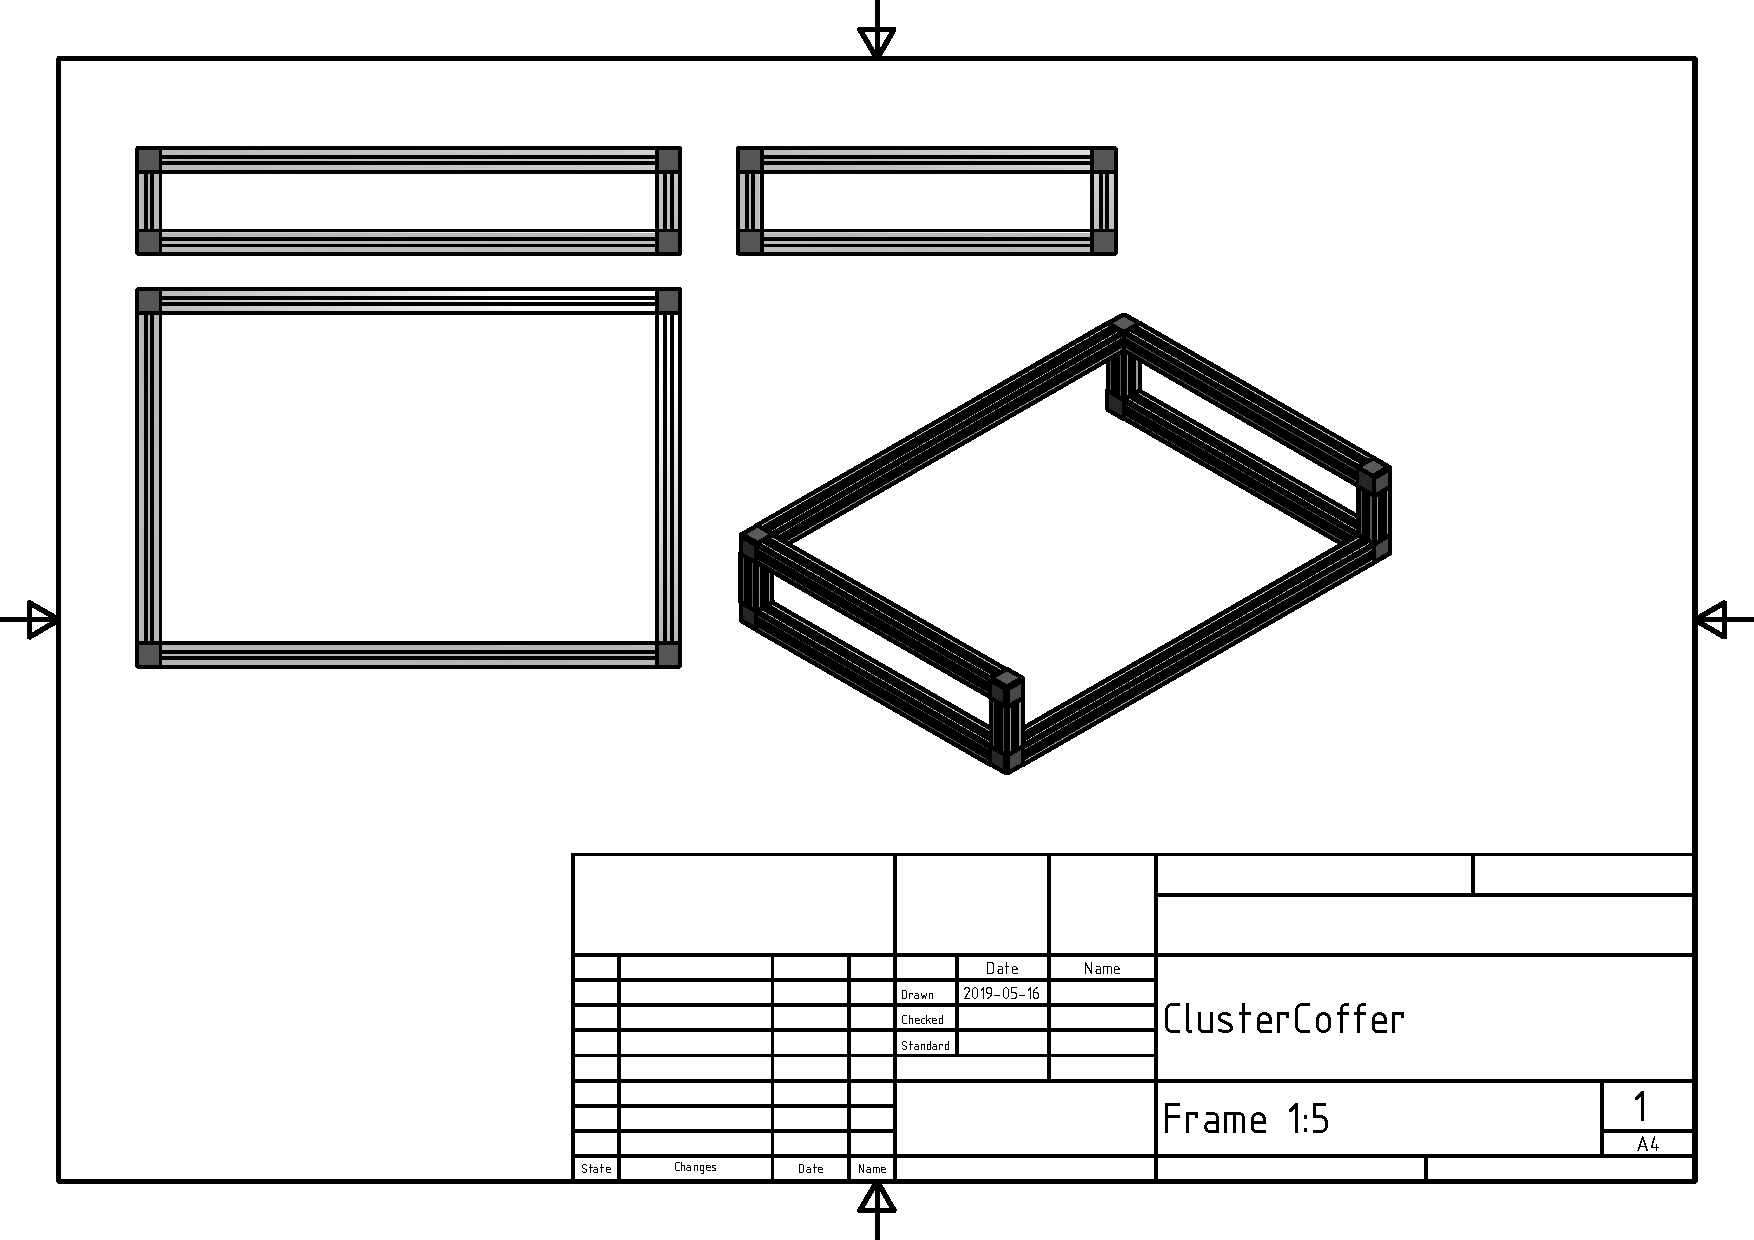
\includepdf[fitpaper]{inc/drawing_frame.pdf}

\section{Base-Plate}

The base-plate is located at the bottom of the assembly.
It holds both power supplies (5 V and 12 V), as well as the switch, and a power conduit box distributing the 230 V mains voltage.

While power supplies and conduit boxes commonly feature mounting holes, the switch requires some gentle modification.
We disassembled the switch and drilled 3 holes into the bottom cover.
This way, it can be mounted to the base-plate using M3 screws.

We also added another hole to the top cover in order to mount a luster terminal.
This comes in handy when wiring up the fans and head node.

The manufacturing drawings at the end of this section are more of a tongue-in-cheek description, but you'll manage.
Holes that belong together are annotated on the same sheet.
The scale is 1:3.

\subsection{Power Supplies}

The beefy 5 V power supply powers the 16 compute nodes.
Head node and fans require 12 V, yet draw considerably less power.

We did not run into any issues with ripple\footnote{\url{https://en.wikipedia.org/wiki/Ripple_(electrical)}}, nevertheless we added capacitors for good measure.
Heat output doesn't seem to be a problem either.

Pay attention to the 230 V terminals of both power supplies.
They should be internal (i.e.\ not accessible from the outside) or at least covered.

\subsection{Switch}

Apart from the 4 new holes, the switch does not feature any other modifications.
The power cord has an angled connector as there is only little clearance between the frame and the mounted switch.
Plug in the power cable before mounting the base-plate to the frame.

\subsection{Mains Power}

Mains power enters the system via a dedicated socket at the back of the case.
This socket also comes with a power switch and a fuse.

On the inside, a cable connects the socket with the conduit box.
The conduit box is connect with the 5 V power supply, the 12 V power supply, and the switch.

Wago-222\footnote{\url{https://www.wago.com/global/installation-terminal-blocks-and-connectors/classic-splicing-connector/p/222-415}} splicing connectors are used.
Large cable ties serve as cable relief.

You can also add additional grounding for the case, frame, or other components if you want.

If any of the components related to 230 V feature open / accessible connectors, consider covering them hot glue.

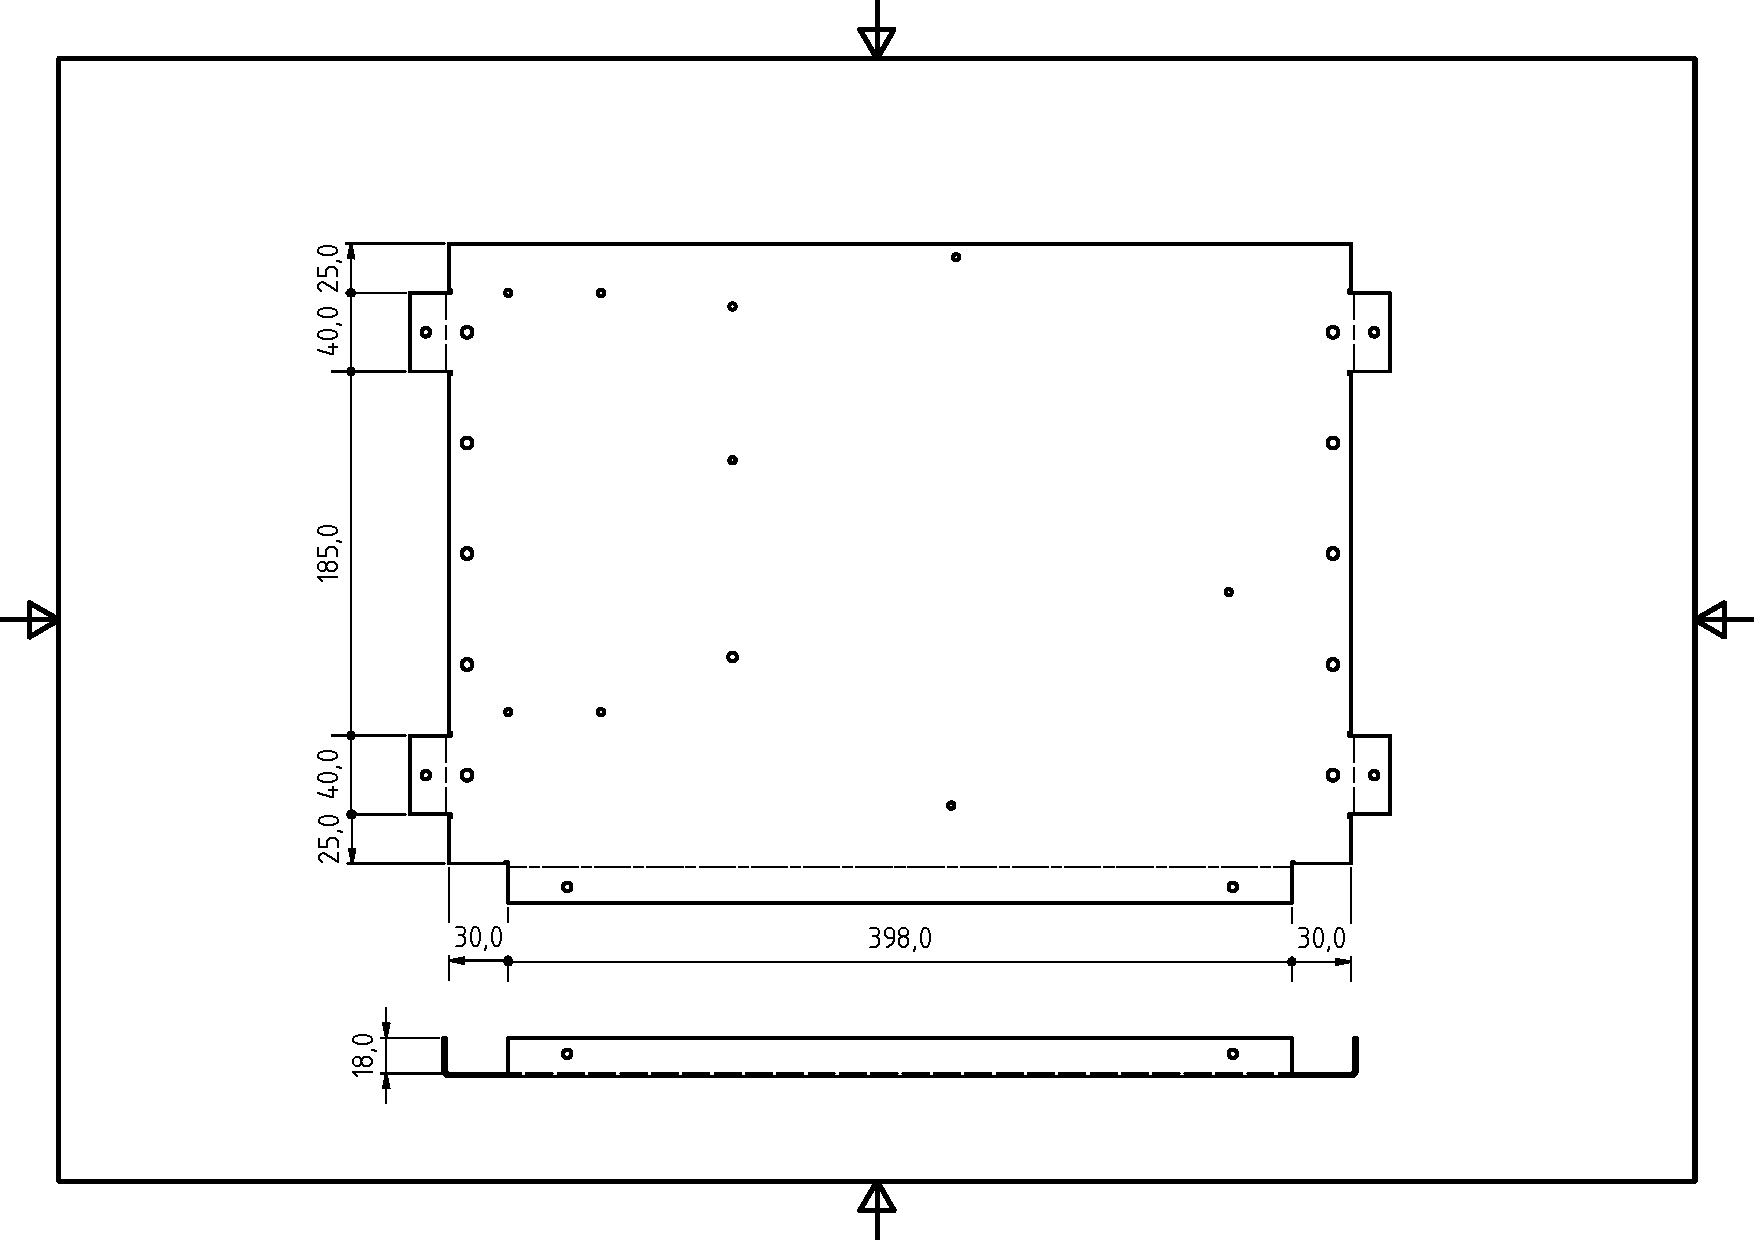
\includepdf[pages=-,fitpaper]{inc/drawing_base_plate.pdf}

\section{V-Mount}

Four V-Mount panels are used to hold all compute nodes.
Each panel holds four compute nodes, four fans, and a power distribution circuit board with switches.

When assembling, start with the fans.
The fans are mounted to the bottom of the panel using countersunk screws.
They push air towards the top, right onto the heatsink.
Ensure the screws sit flush with the surface to prevent any gaps through which air could escape the heatsinks.

The heatsinks of the compute nodes already come with M3 mounting holes that are used for mounting them to the panel.

Consider dealing with the software stuff before mounting them to the panel, as it will be cumbersome to access the micro SD card afterwards.

The power distribution circuit board is added next.
The only mechanical connection is the four toggle switches; however, as there shouldn't be any stress on the board, this should be fine.
Try not to scratch the surface of the panel when tightening the nuts.

After everything has been mounted to the panel, it is recommended to start cable management.
Start by connecting the fan power cables to the power distribution board.
After that, the custom compute node power boards can be attached.

The scale of the following design documents is 1:2.

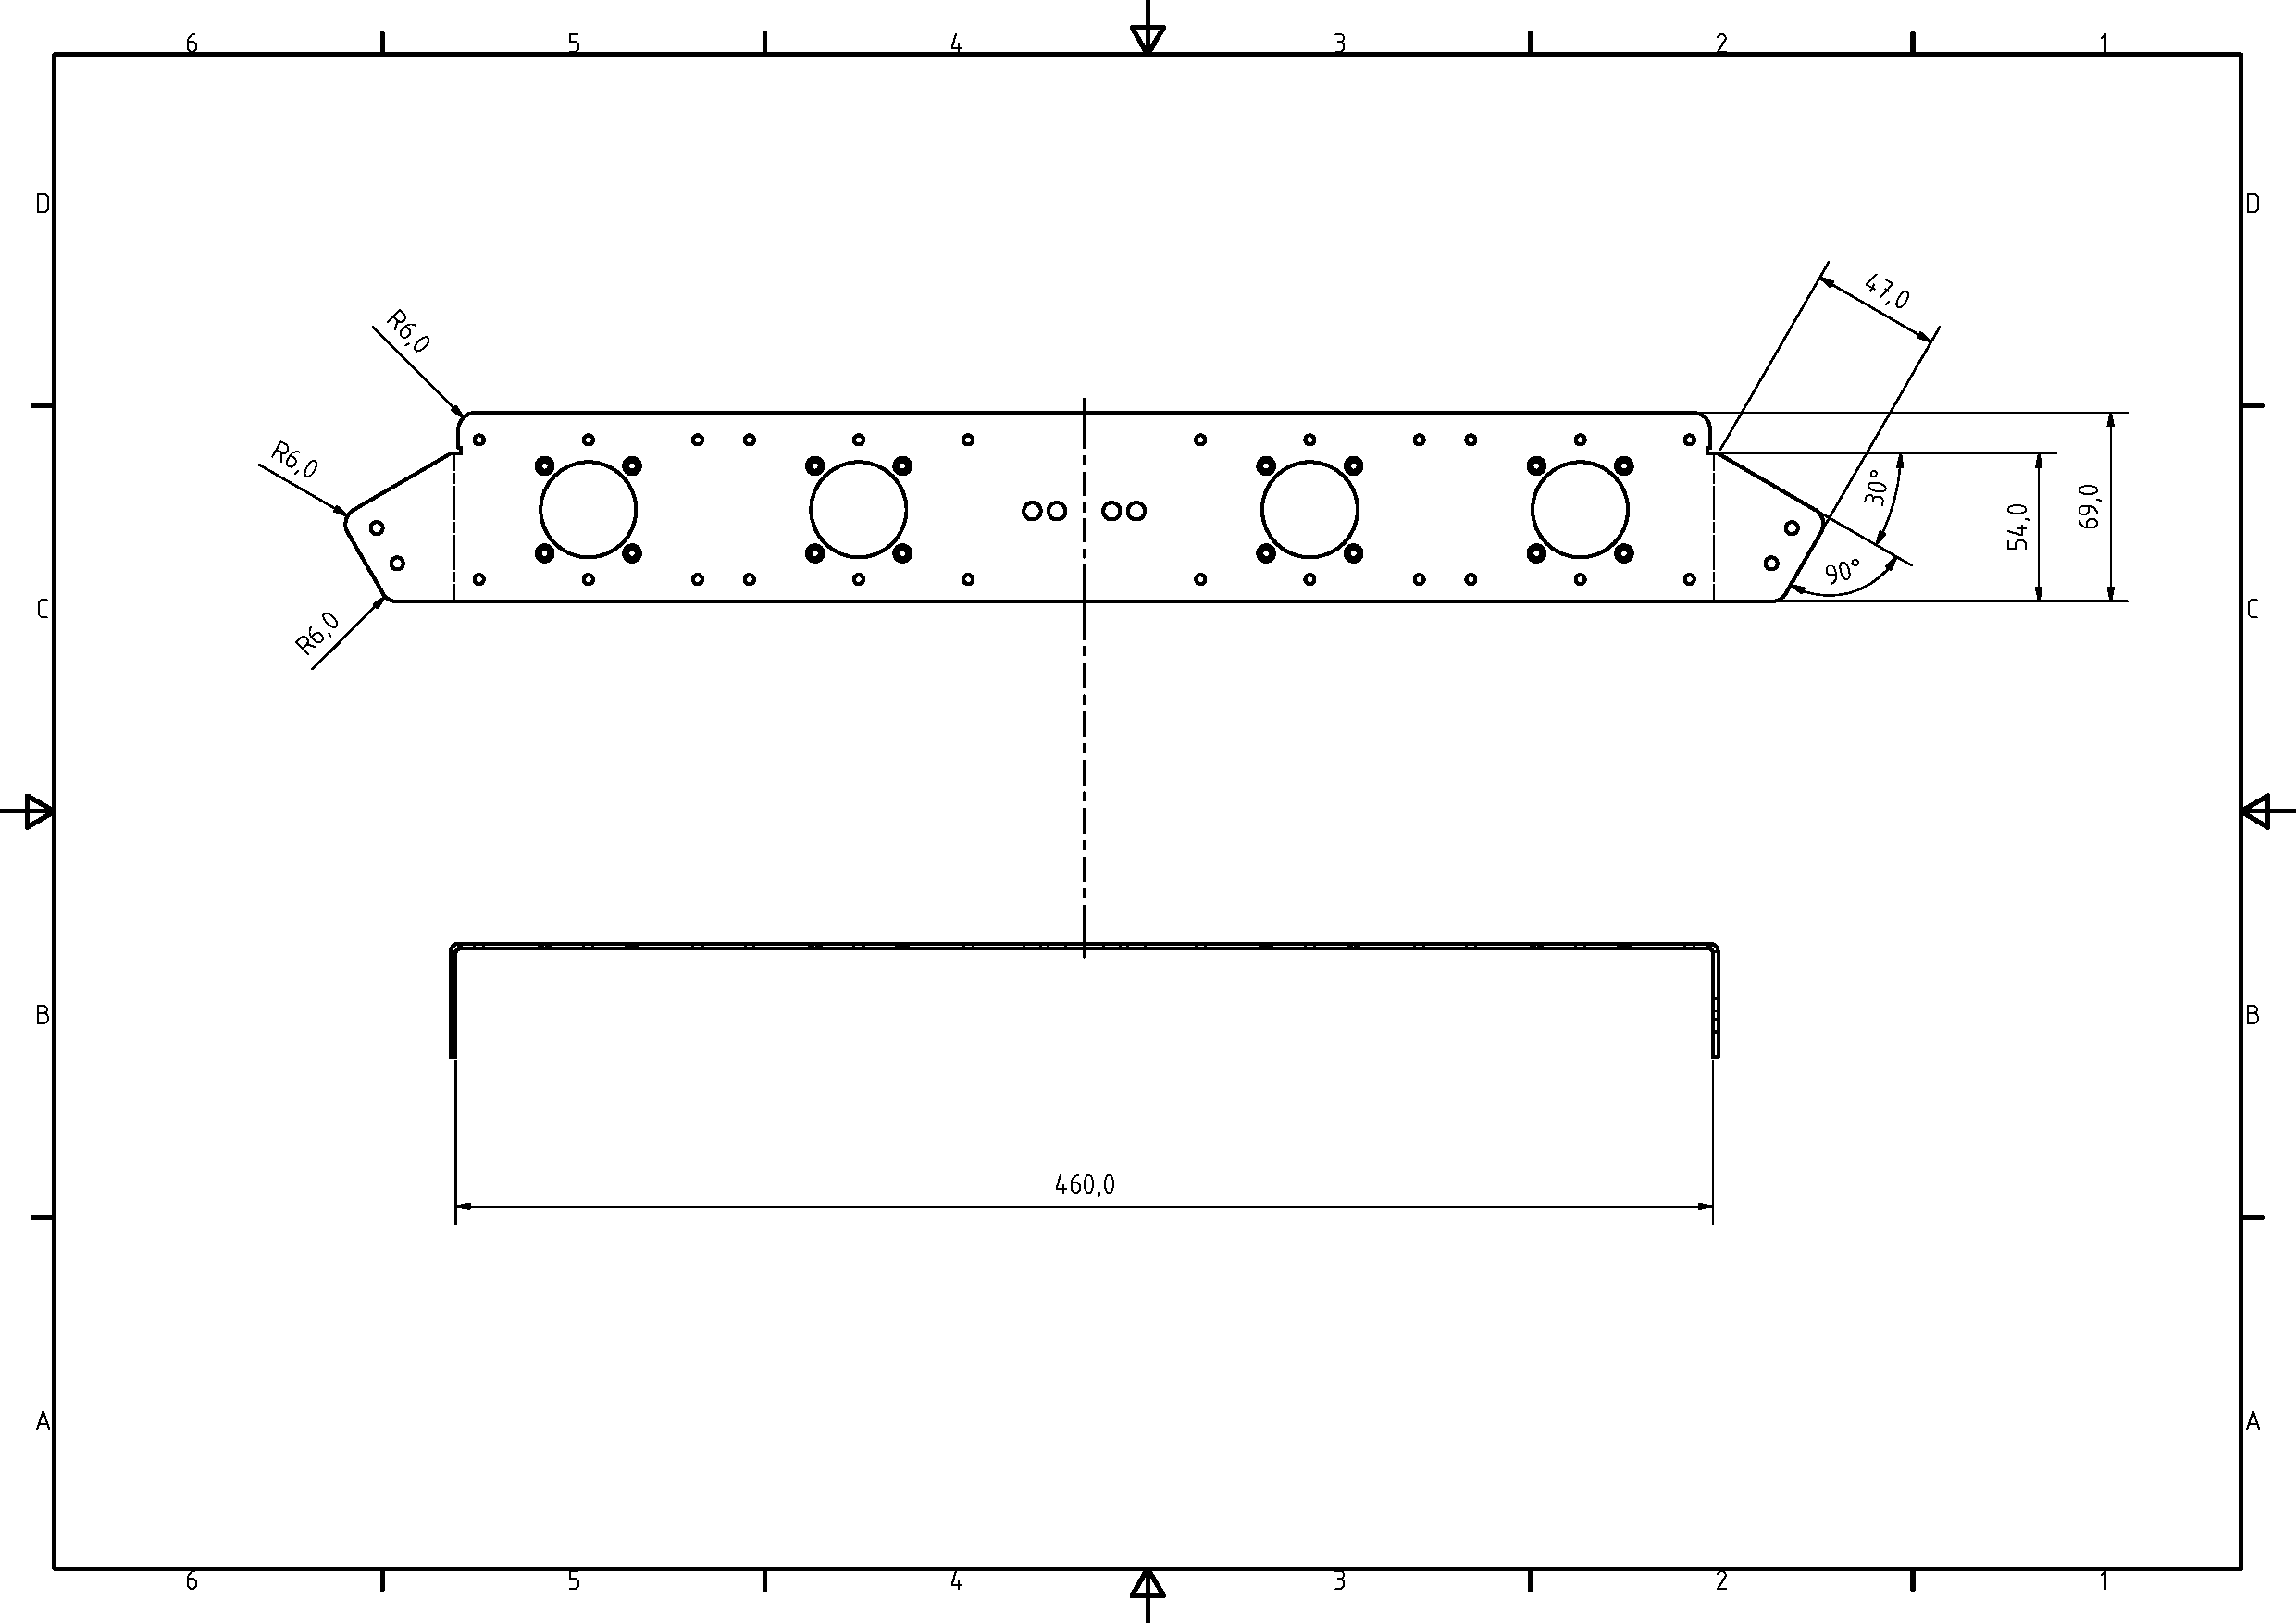
\includepdf[pages=-,fitpaper]{inc/drawing_v_mount.pdf}

\chapter{Electronics}

This chapter describes the electronic components.
The head node and compute nodes are off-the-shelf embedded systems and require little to no hardware related modifications.

There are 2 custom PCB designs: the compute node power board (\textit{ccpad}) and the panel power distribution board (\textit{ccpdu}).

Software:

\begin{itemize}
	\item \href{http://kicad-pcb.org/}{KiCad}
\end{itemize}

\section{NanoPC-T4}

See \url{https://www.friendlyarm.com/index.php?route=product/product&product_id=225}.

\section{NanoPi M4 2 GB}

See \url{https://www.friendlyarm.com/index.php?route=product/product&product_id=234}.

\section{ccpad}

The main purpose of a ccpad is to supply a compute node with power.
While a compute node can be powered via USB Type-C, the USB Type-C cables / connectors are relatively expensive and their length make them non-ideal for this build.

A ccpad has an input terminal for 5 V and is connected directly to the pin header of a compute board.
This setup also allows for a power measurement IC to be added \emph{and connected} to a compute board.

An \textit{INA219 Zero-Drift, Bidrectional Current/Power Monitor with I²C Interface} is used.

Pin header connector and input terminal are installed on \emph{the same side}.

Consider covering up the bottom of the board with hot glue to prevent short circuits with the adjacent V-Mount panel when fully assembled.

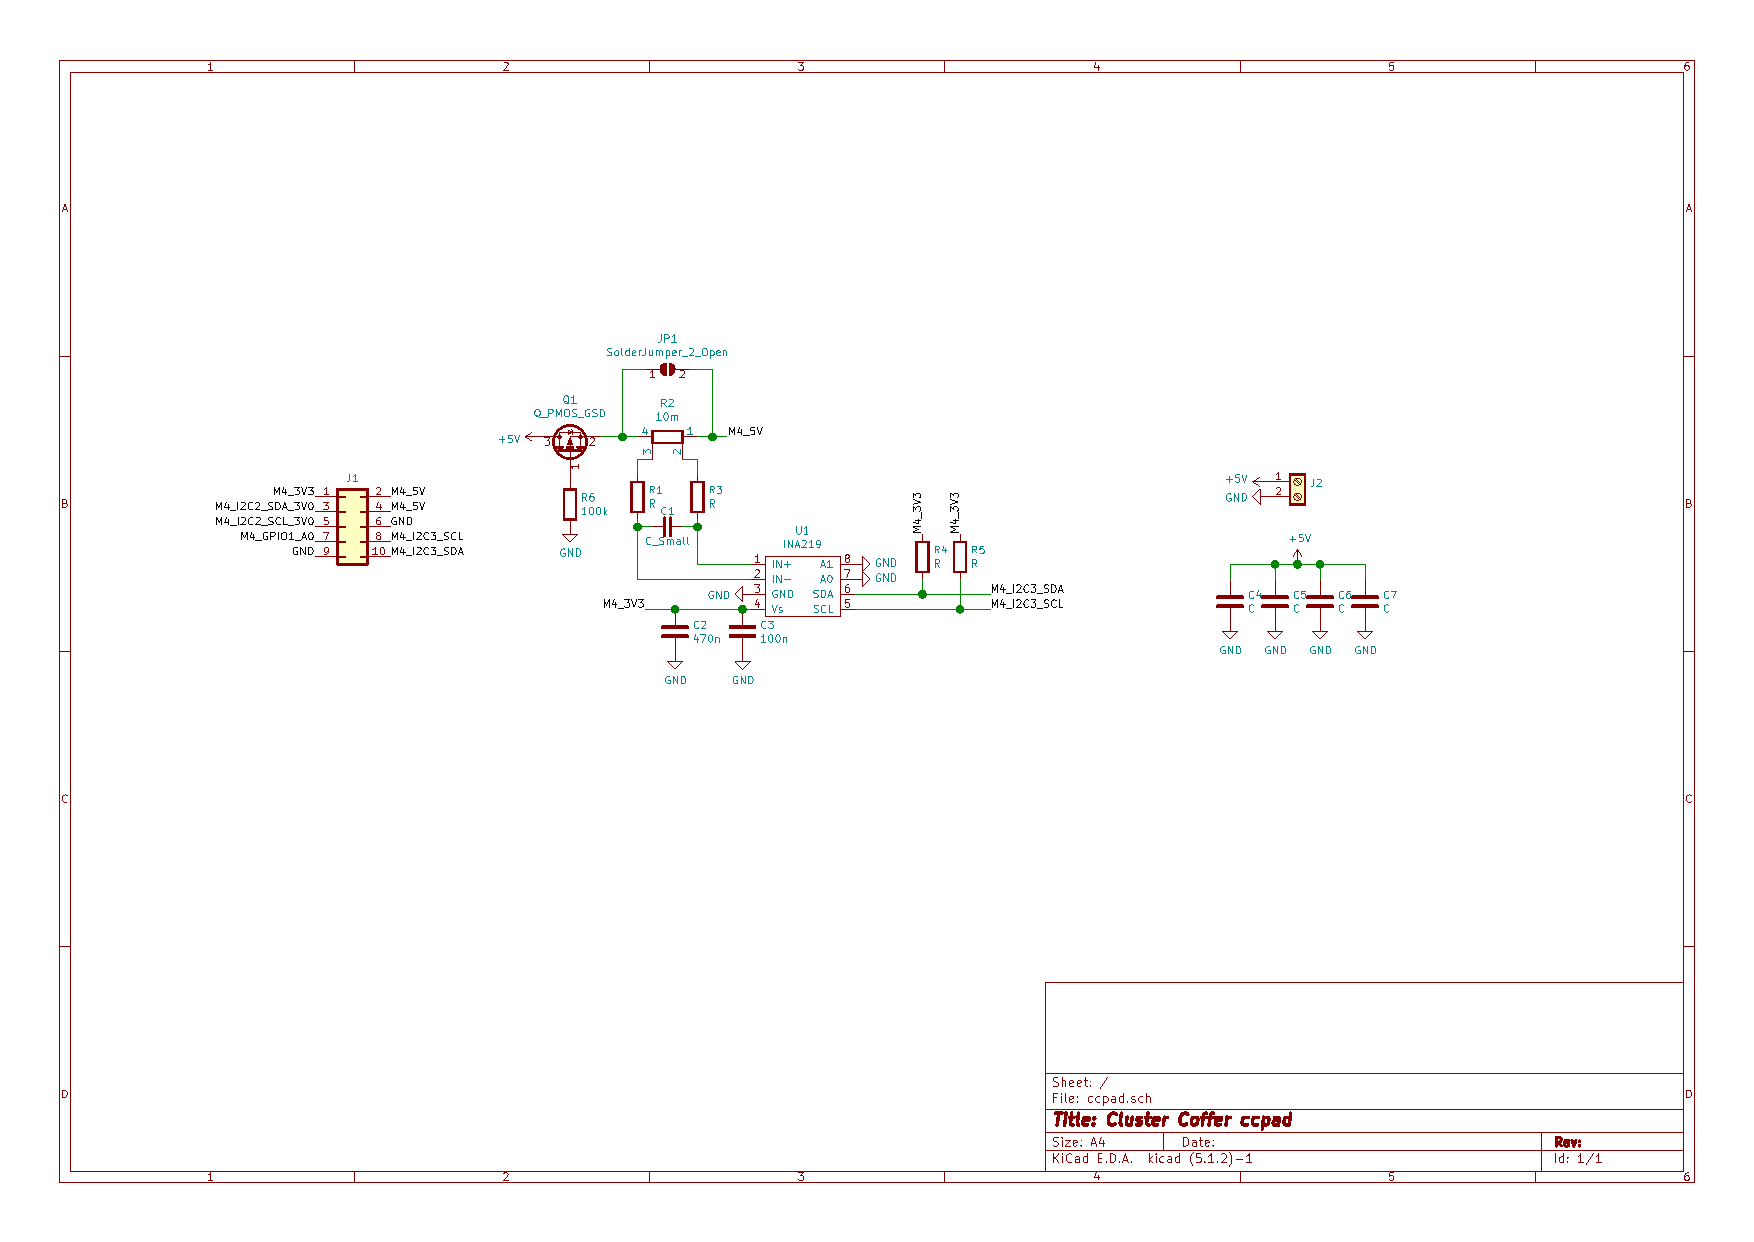
\includepdf[fitpaper]{inc/ccpad_schematic.pdf}
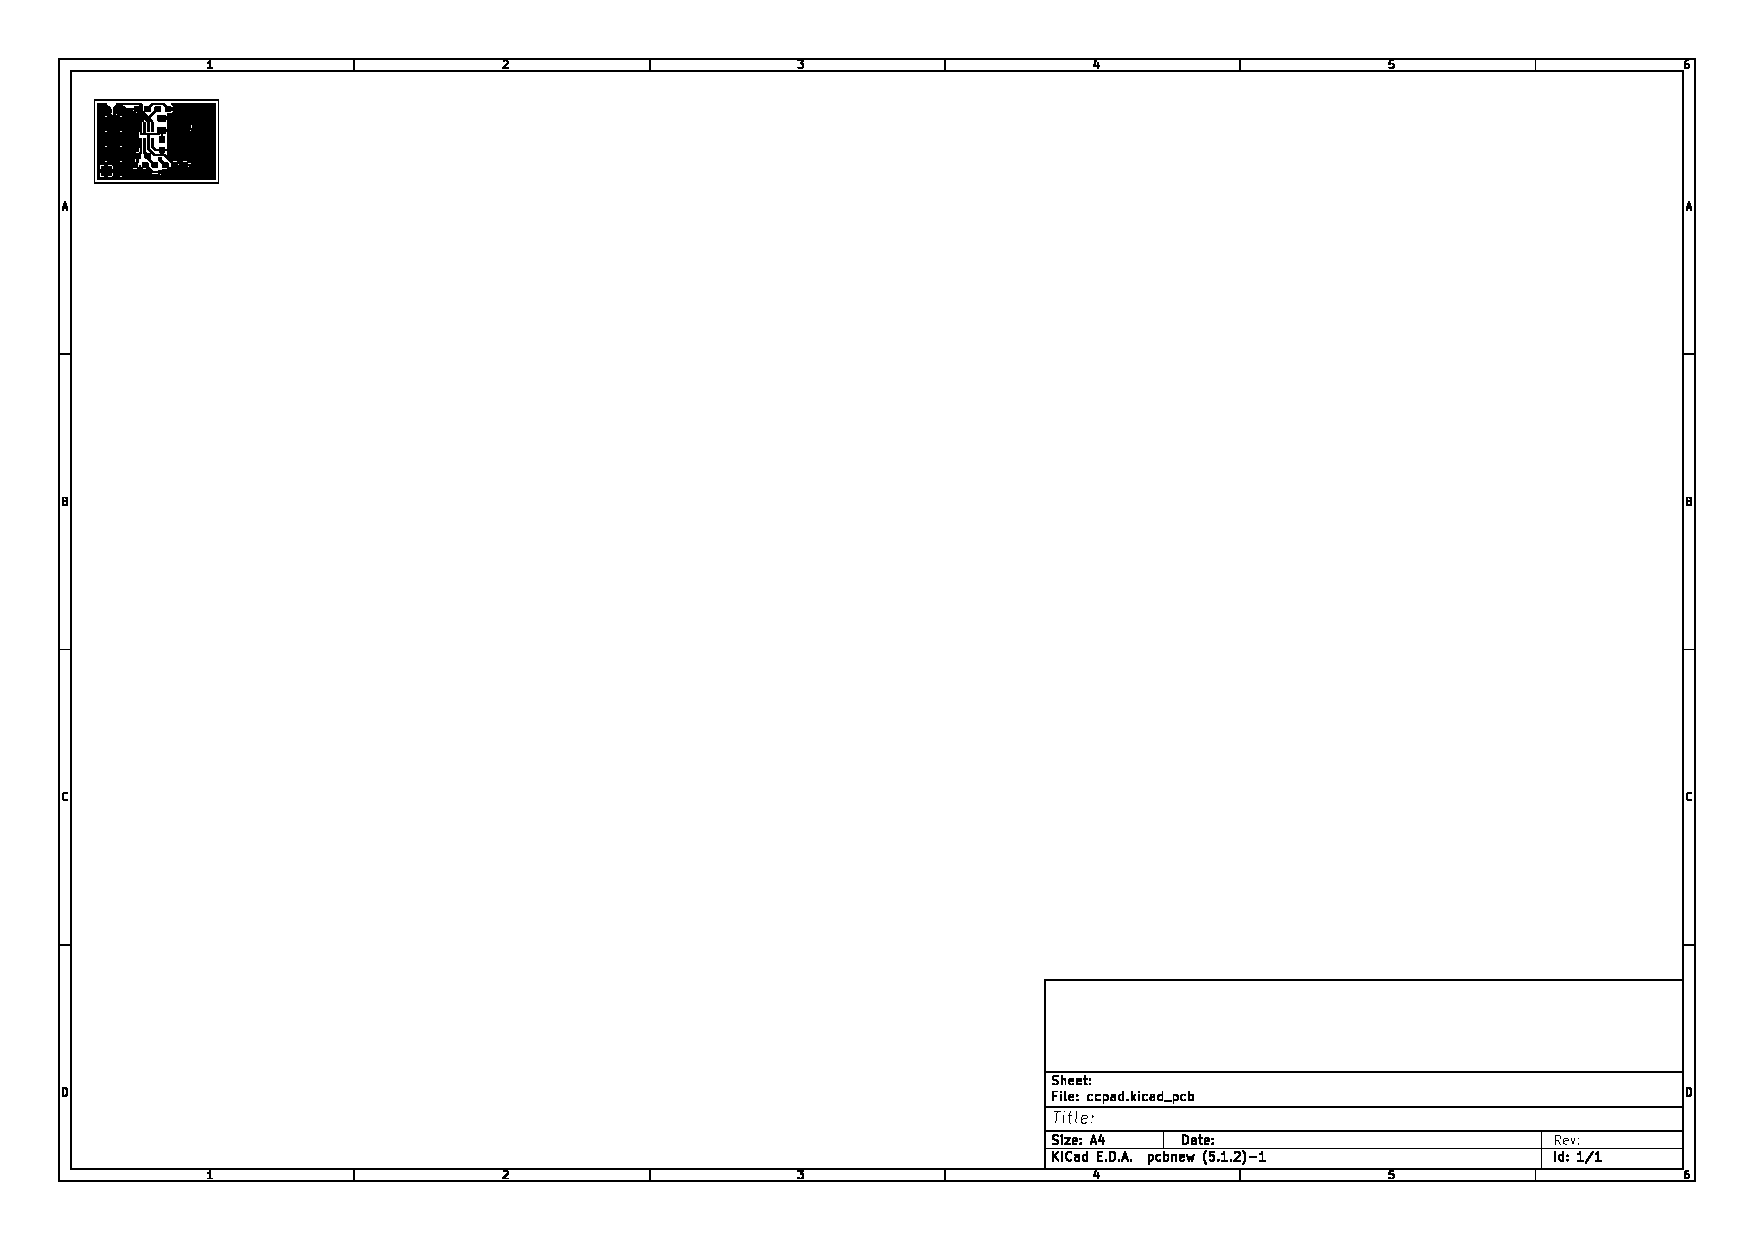
\includepdf[fitpaper]{inc/ccpad_top.pdf}
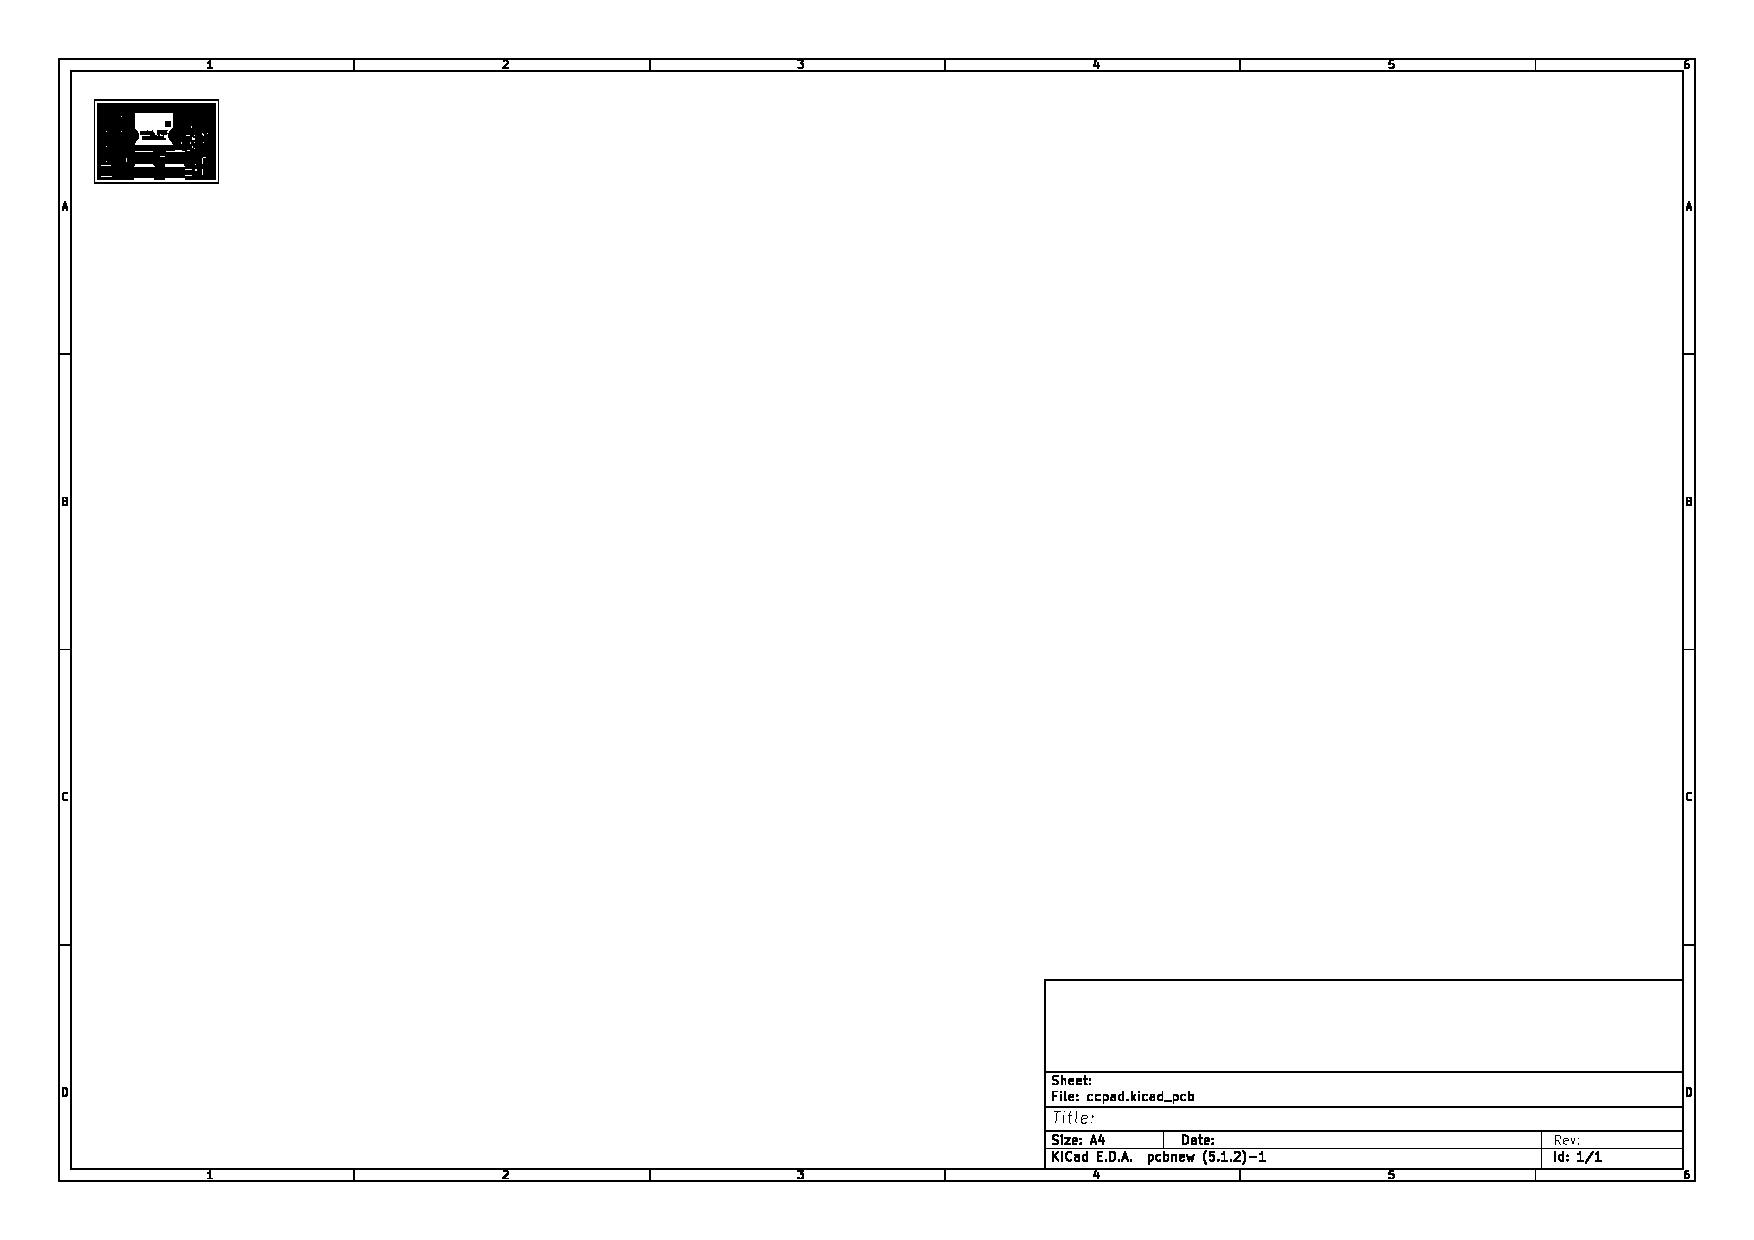
\includepdf[fitpaper]{inc/ccpad_bottom.pdf}
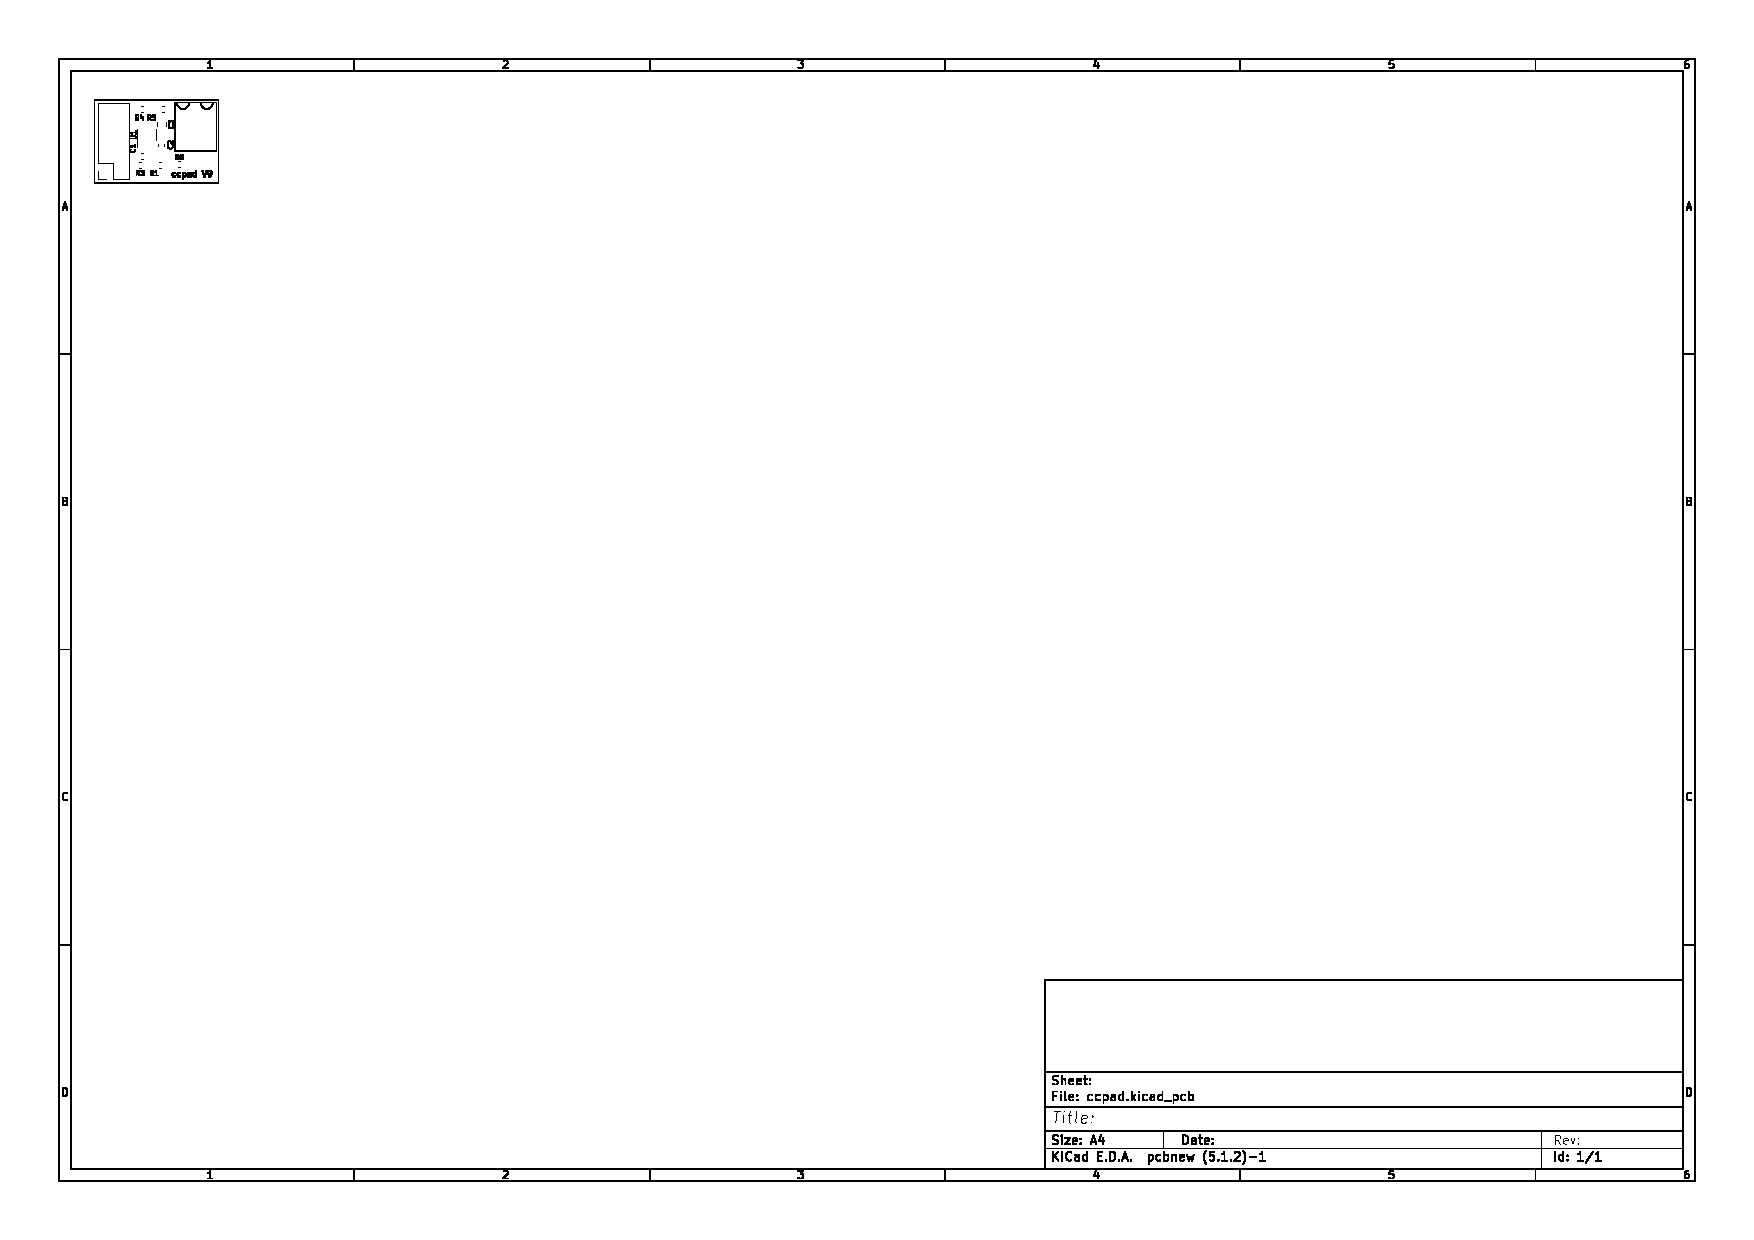
\includepdf[fitpaper]{inc/ccpad_silk.pdf}
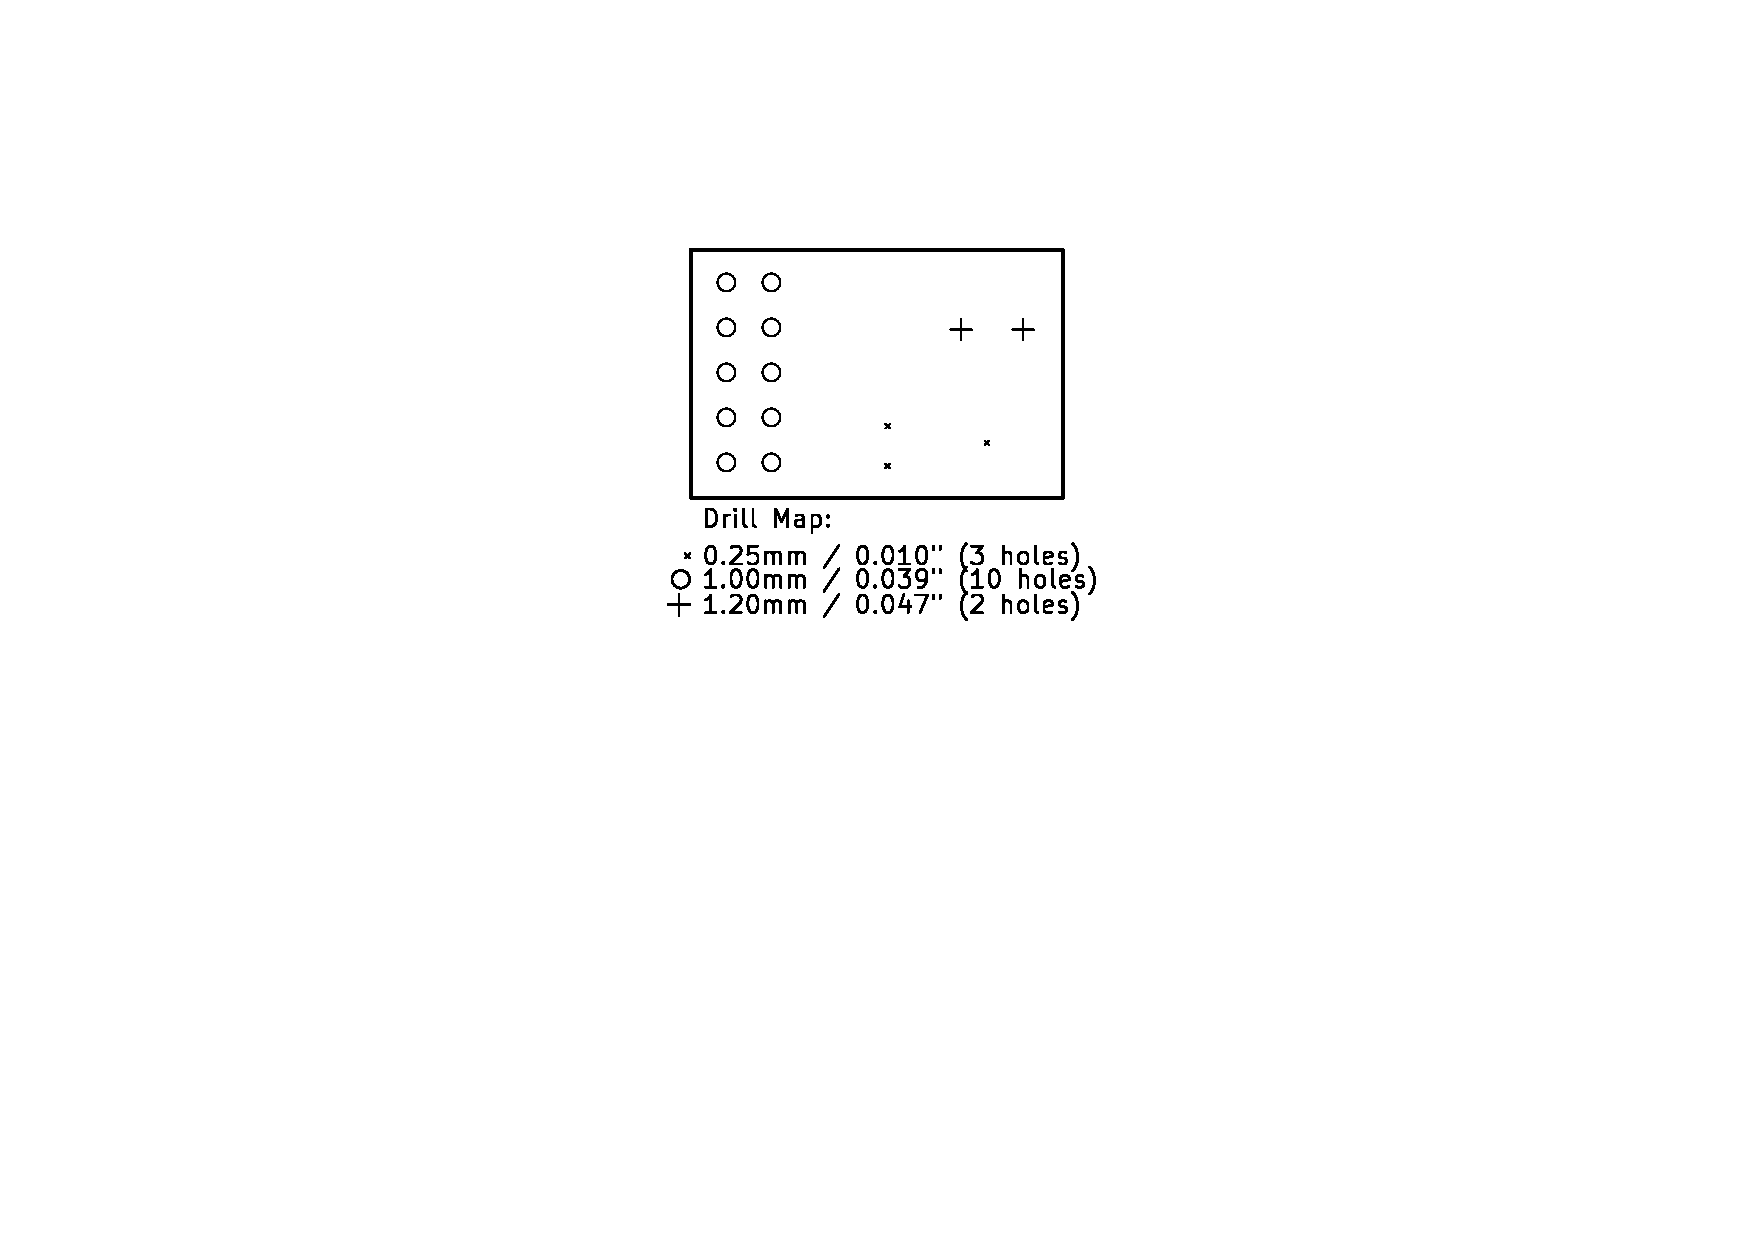
\includepdf[fitpaper]{inc/ccpad_drill.pdf}

\section{ccpdu}

The ccpdu serves as a power distribution board.
While the fans run with 12 V, the compute nodes require 5 V.

The four toggle switches per board are used to mechanically mount it to the V-Mount panel.
Switches and terminals are installed on \emph{opposite sides}.

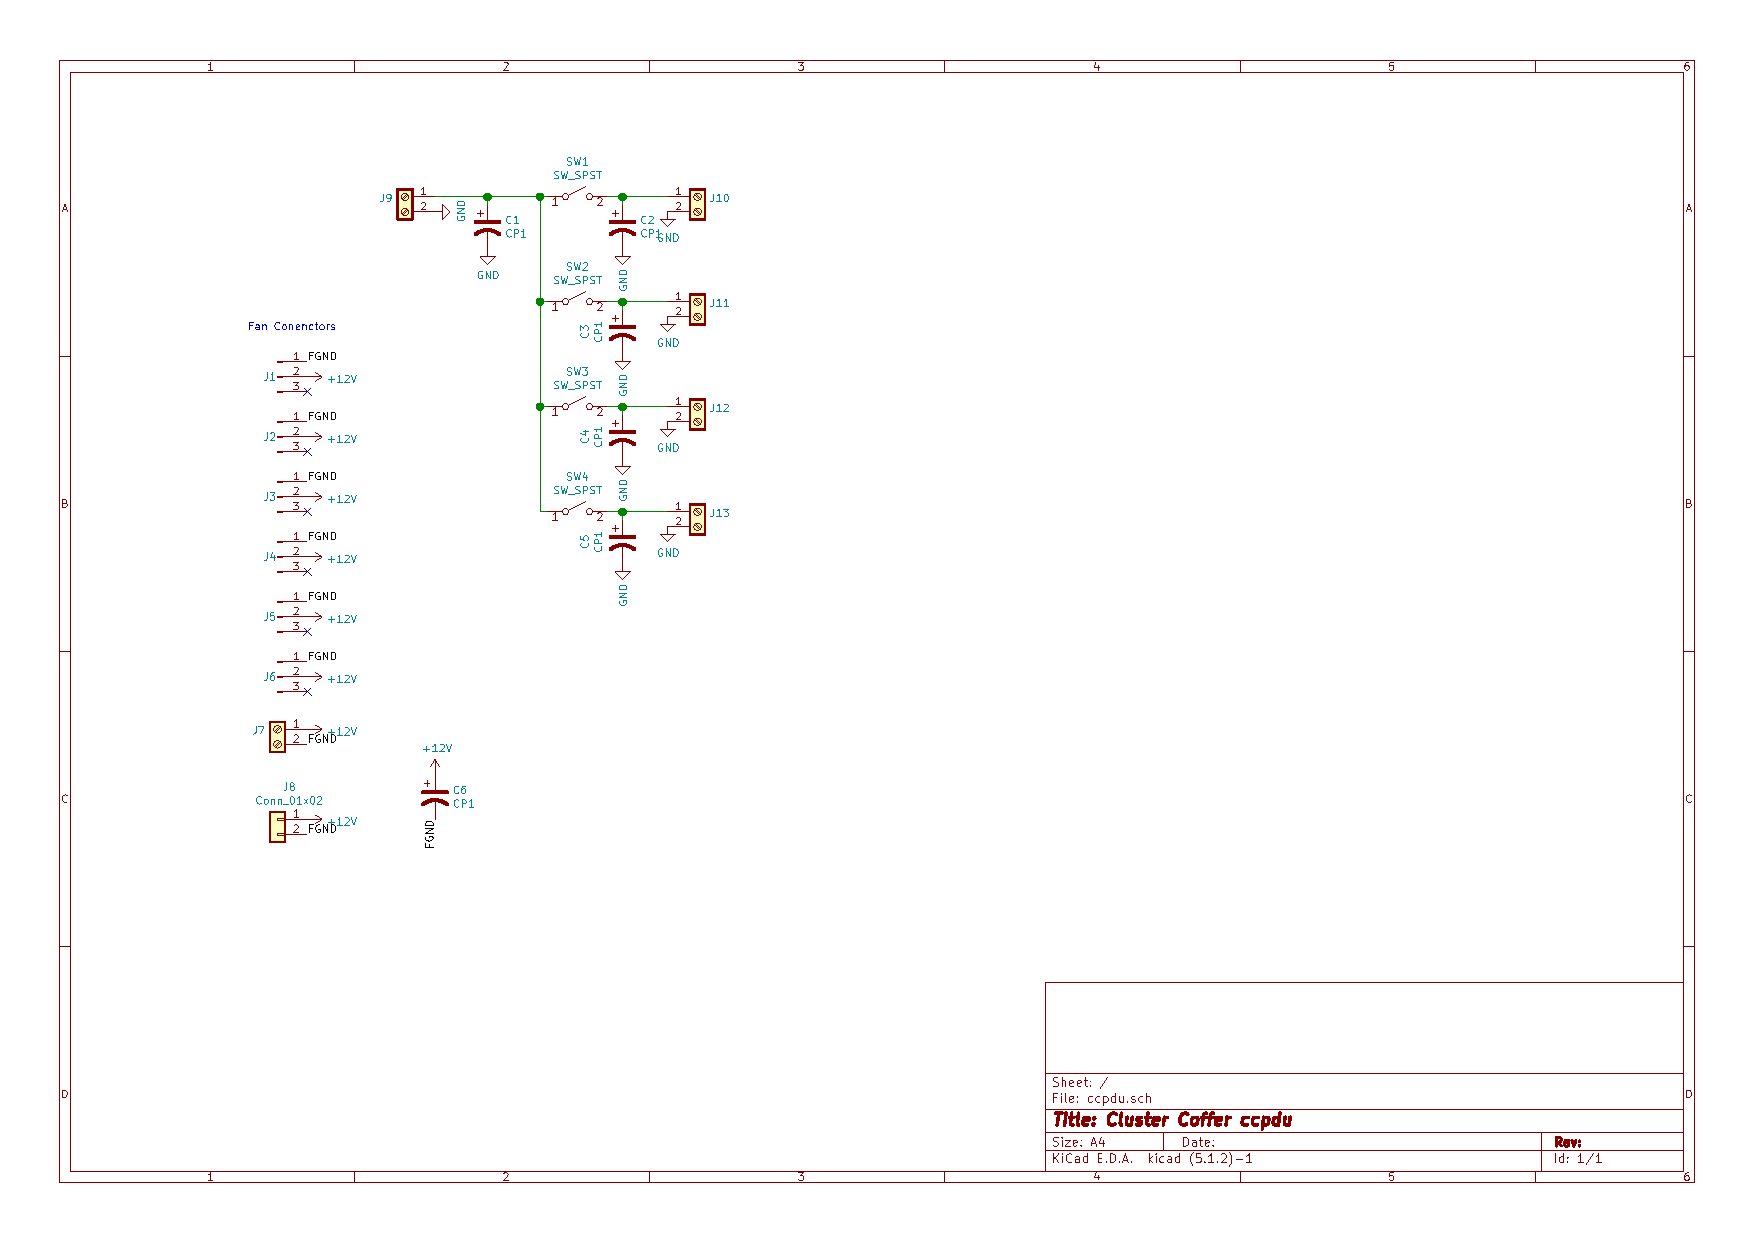
\includepdf[fitpaper]{inc/ccpdu_schematic.pdf}
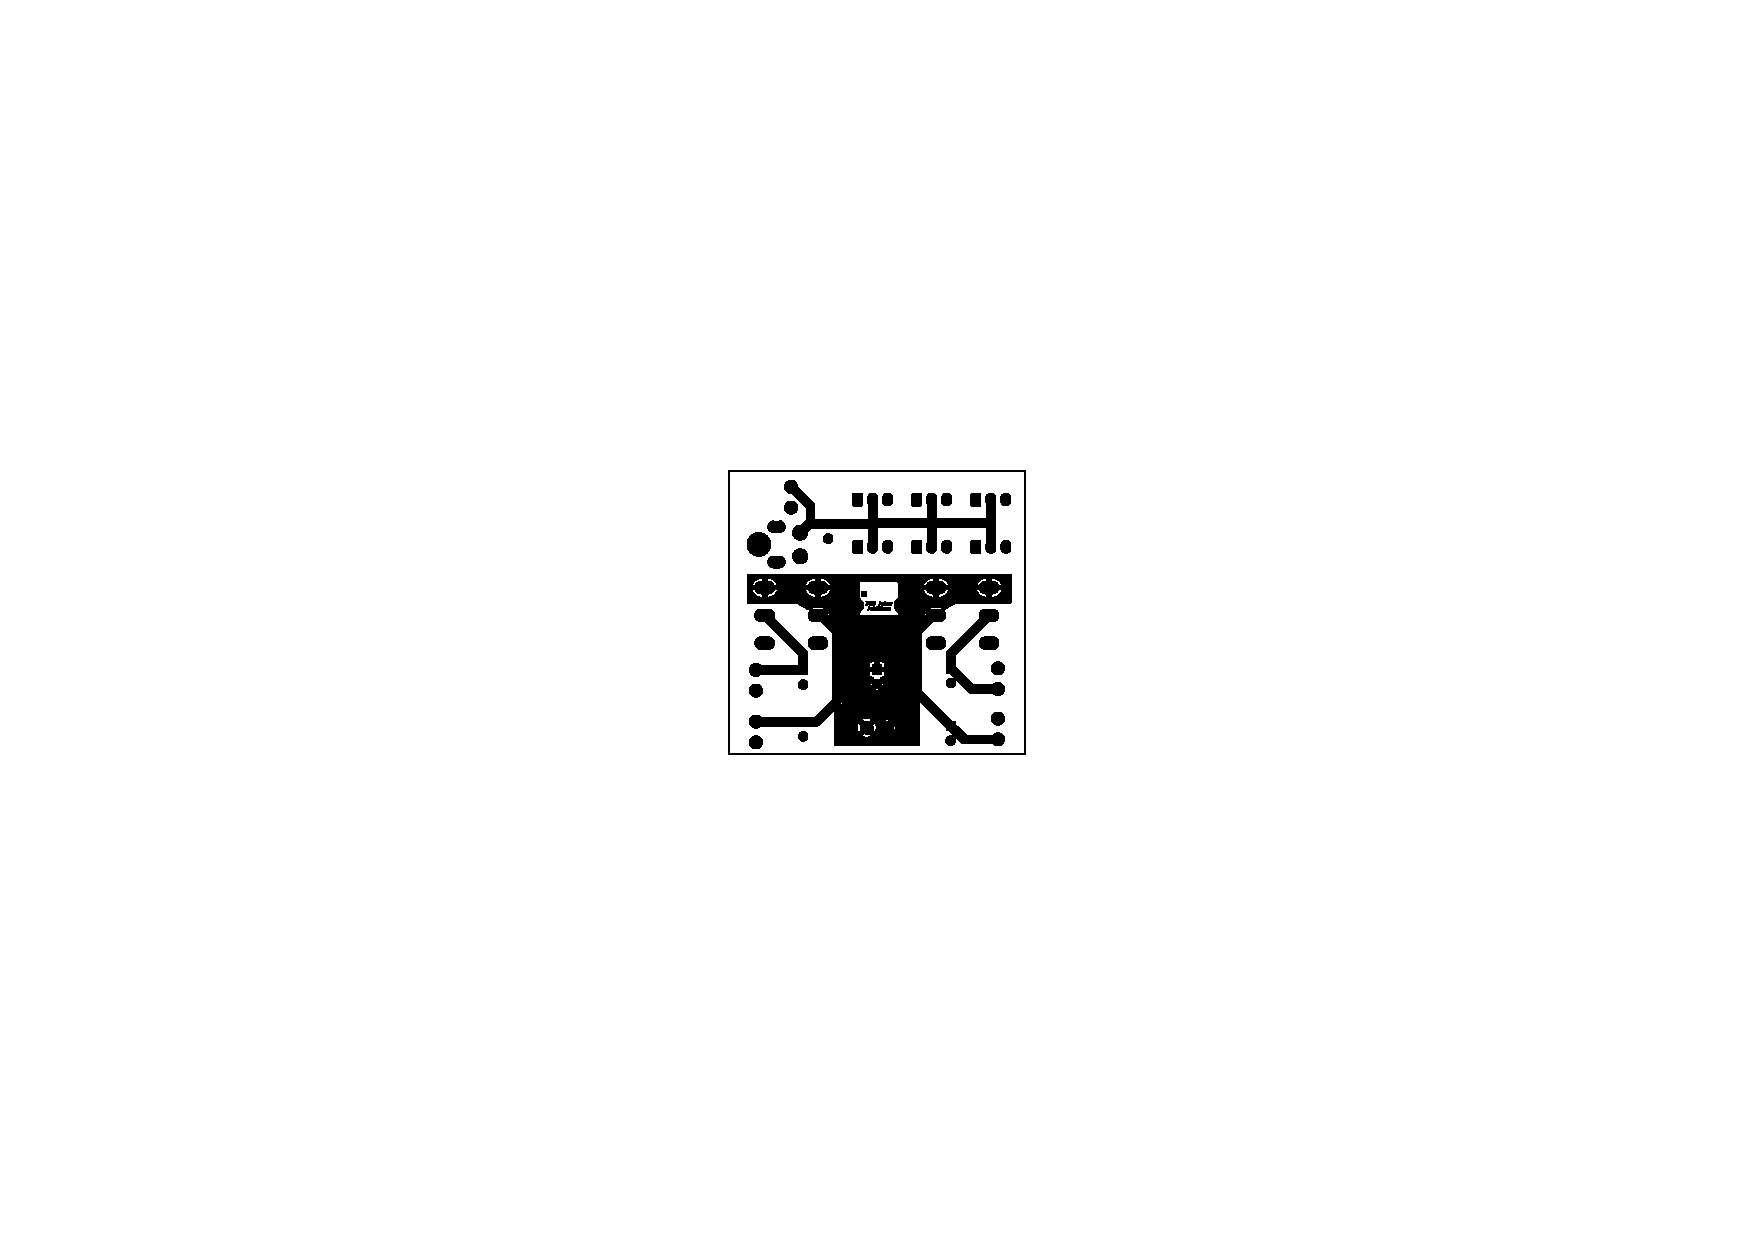
\includepdf[fitpaper]{inc/ccpdu_top.pdf}
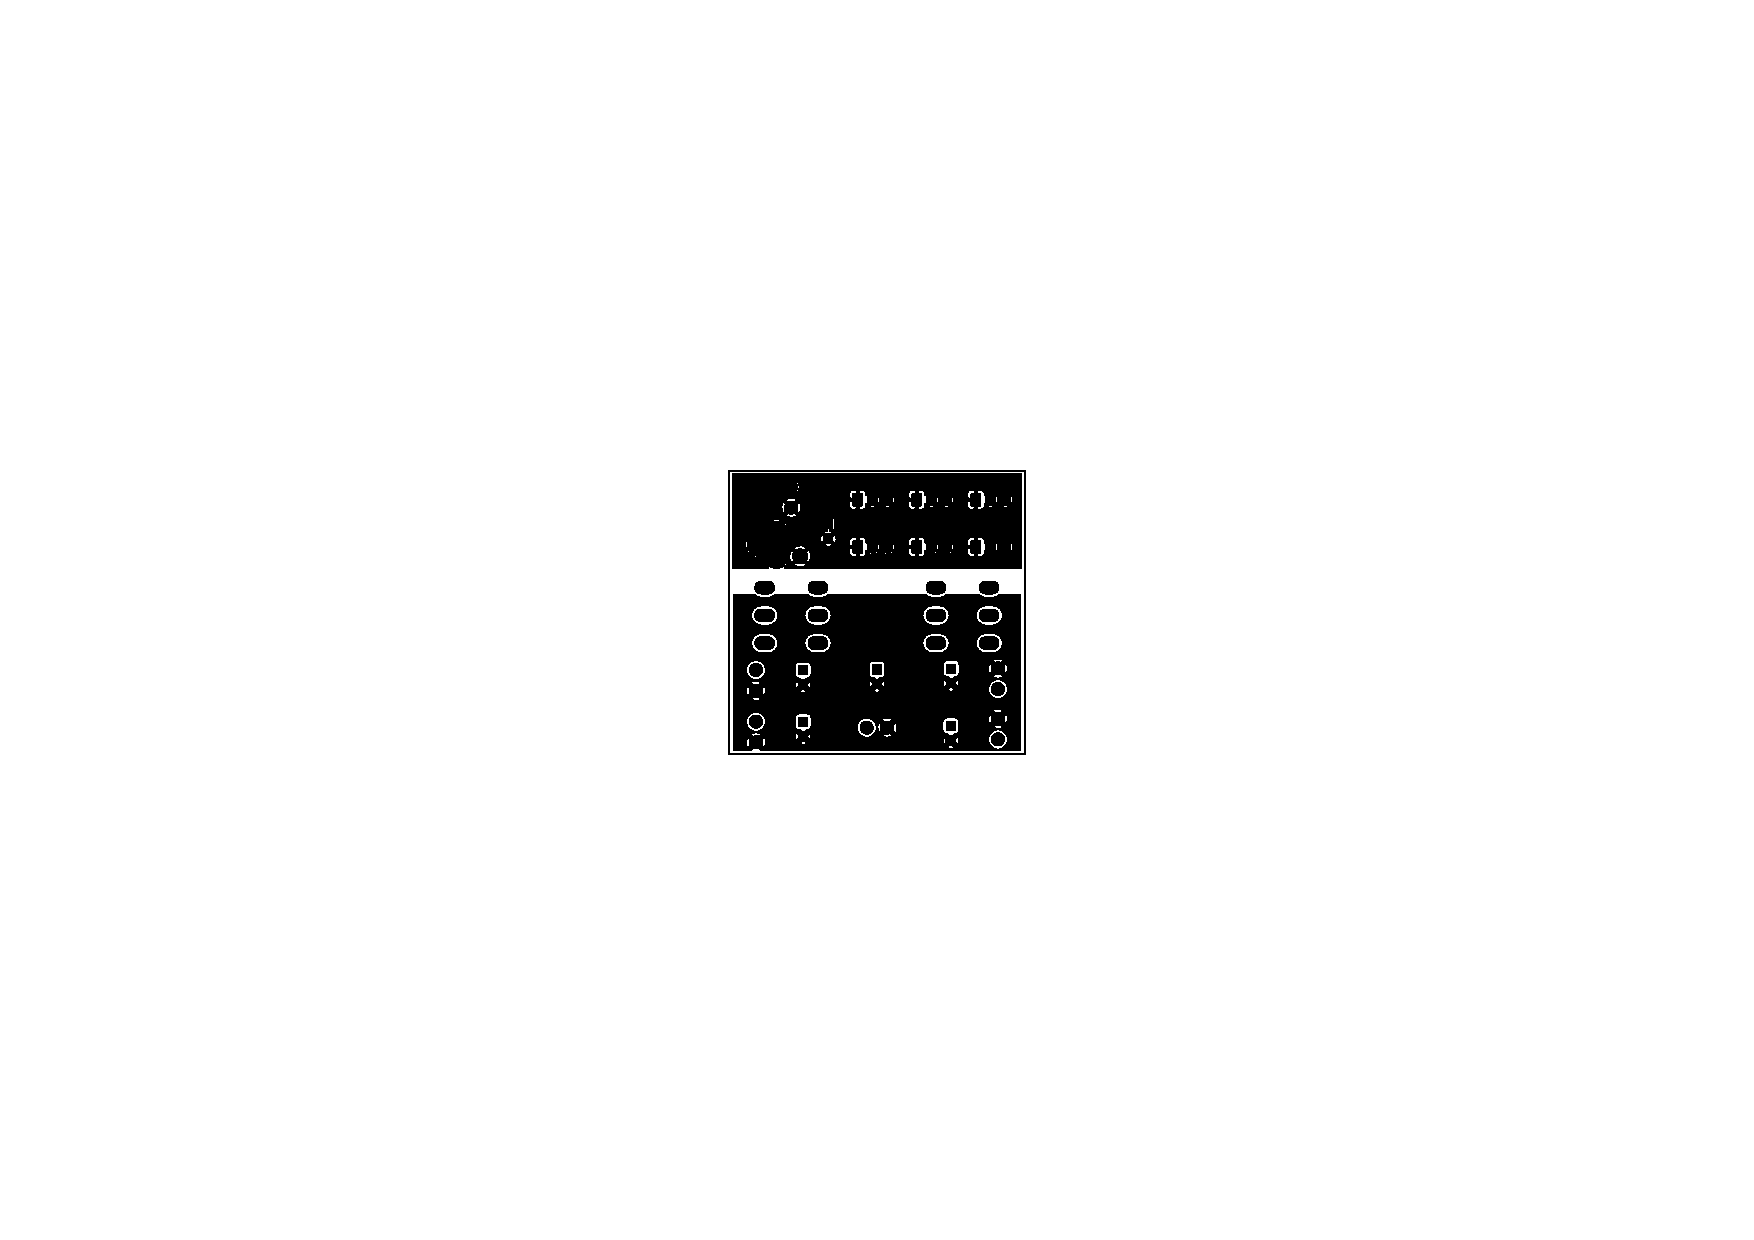
\includepdf[fitpaper]{inc/ccpdu_bottom.pdf}
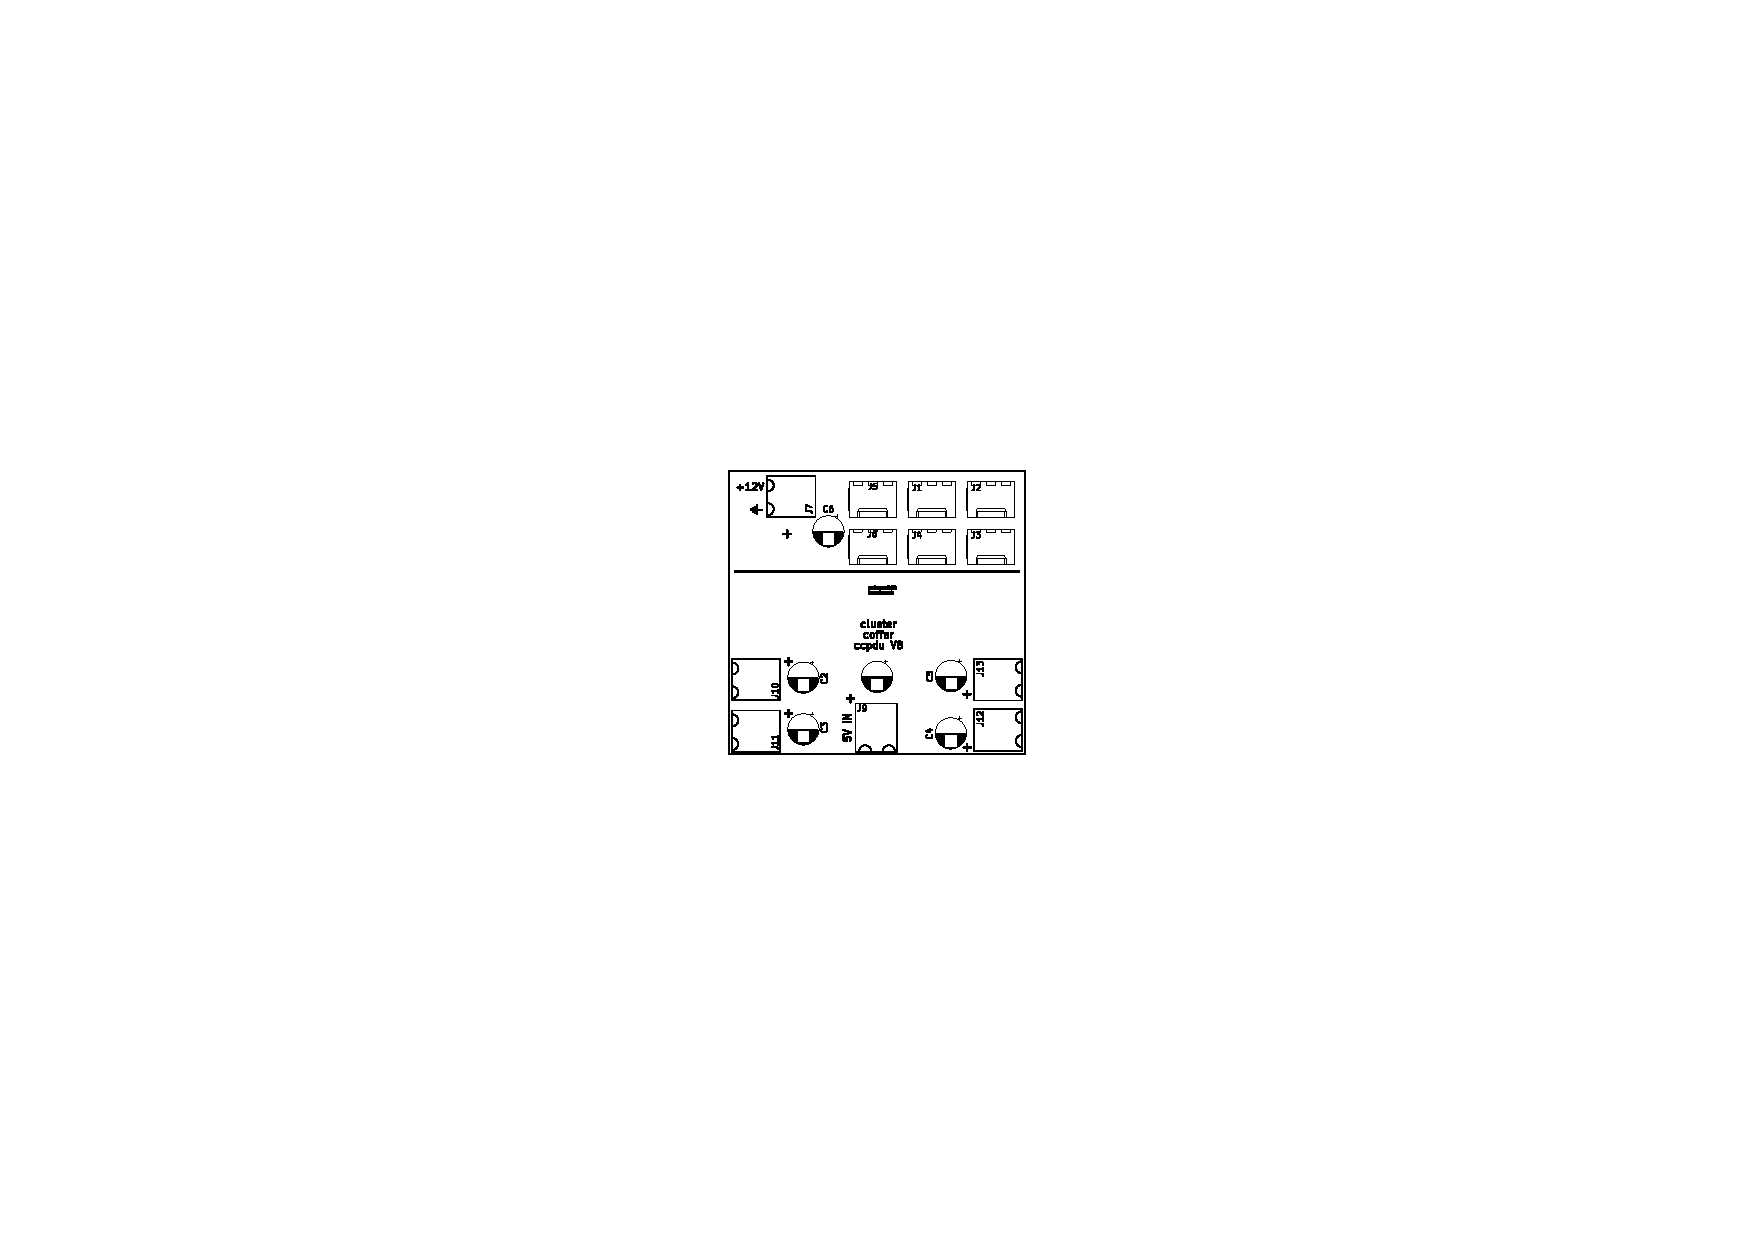
\includepdf[fitpaper]{inc/ccpdu_silk.pdf}
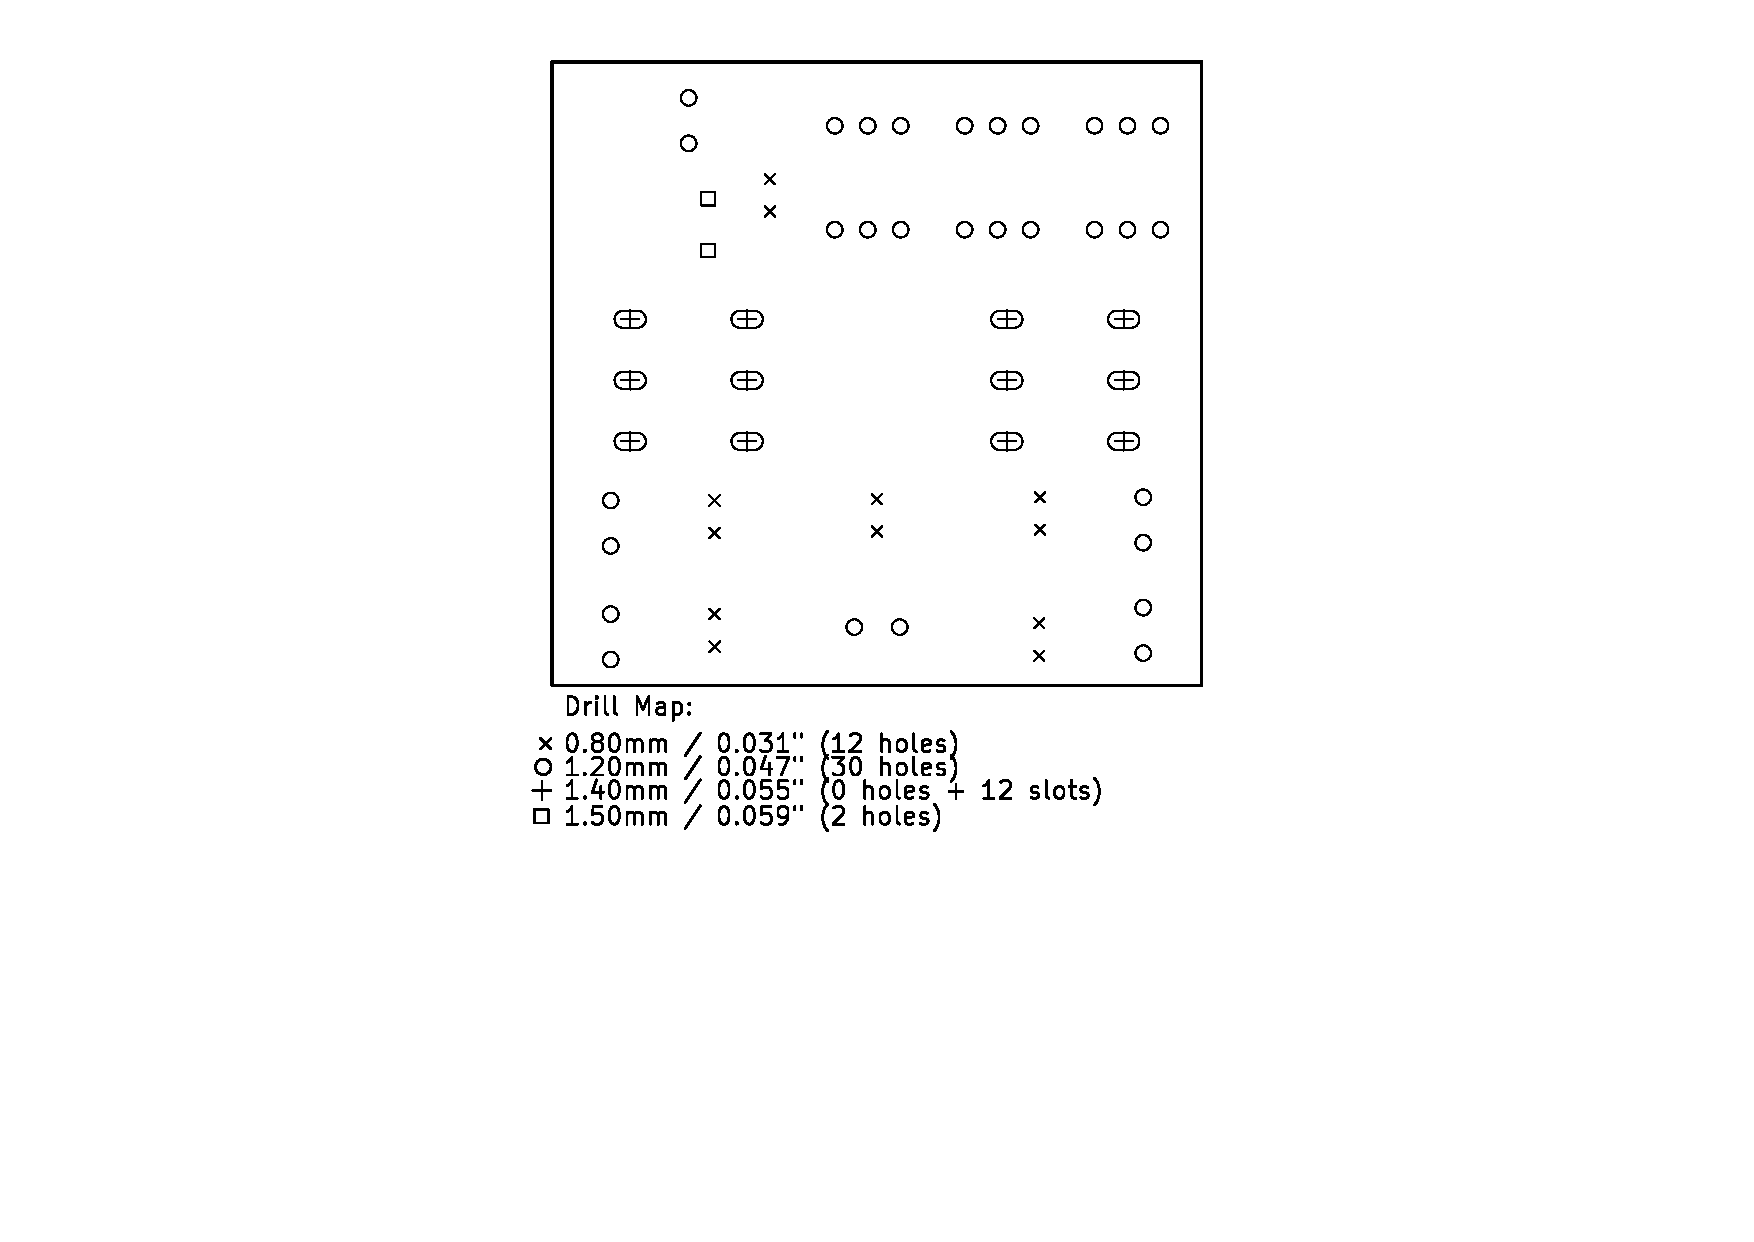
\includepdf[fitpaper]{inc/ccpdu_drill.pdf}

\chapter{Software}

This chapter explains the software setup of the head and compute nodes.

Software:

\begin{itemize}
	\item \href{https://www.denx.de/wiki/U-Boot}{U-Boot}
	\item \href{https://www.debian.org/}{Debian}
\end{itemize}

\section{Head Node}

As OS a custom Debian image is used and stored on the SD card.
U-Boot, also present on the SD card, is used as bootloader.
The project repository contains a collection of scripts which builds the bootloader and image for you.

All compute nodes are listed in the head node's hosts file.
It's IP address is static.
It runs a DHCP service for the compute nodes.

A service writes the \texttt{authorized\_keys} file for the compute nodes.

At the point of writing we did not manage to get the M.2 SSD drive to work.

\section{Compute Node}

The compute nodes use U-Boot as bootloader on their SD cards.
However, the OS image is located in the head node's eMMC memory and loaded via TFTP.
The head node's IP address and kernel image path are hardcoded in U-Boot.

All compute nodes share the same OS image, which is mounted read-only.
OverlayFS is used to enable writing.
All changes are stored in RAM, hence they are lost on reboot.

IPs are determined via DHCP.

\subsection{INA219}

The power measurement values can be read from somewhere in \texttt{/sys/class/hwmon}.

\chapter{Gallery}

\begin{figure}
	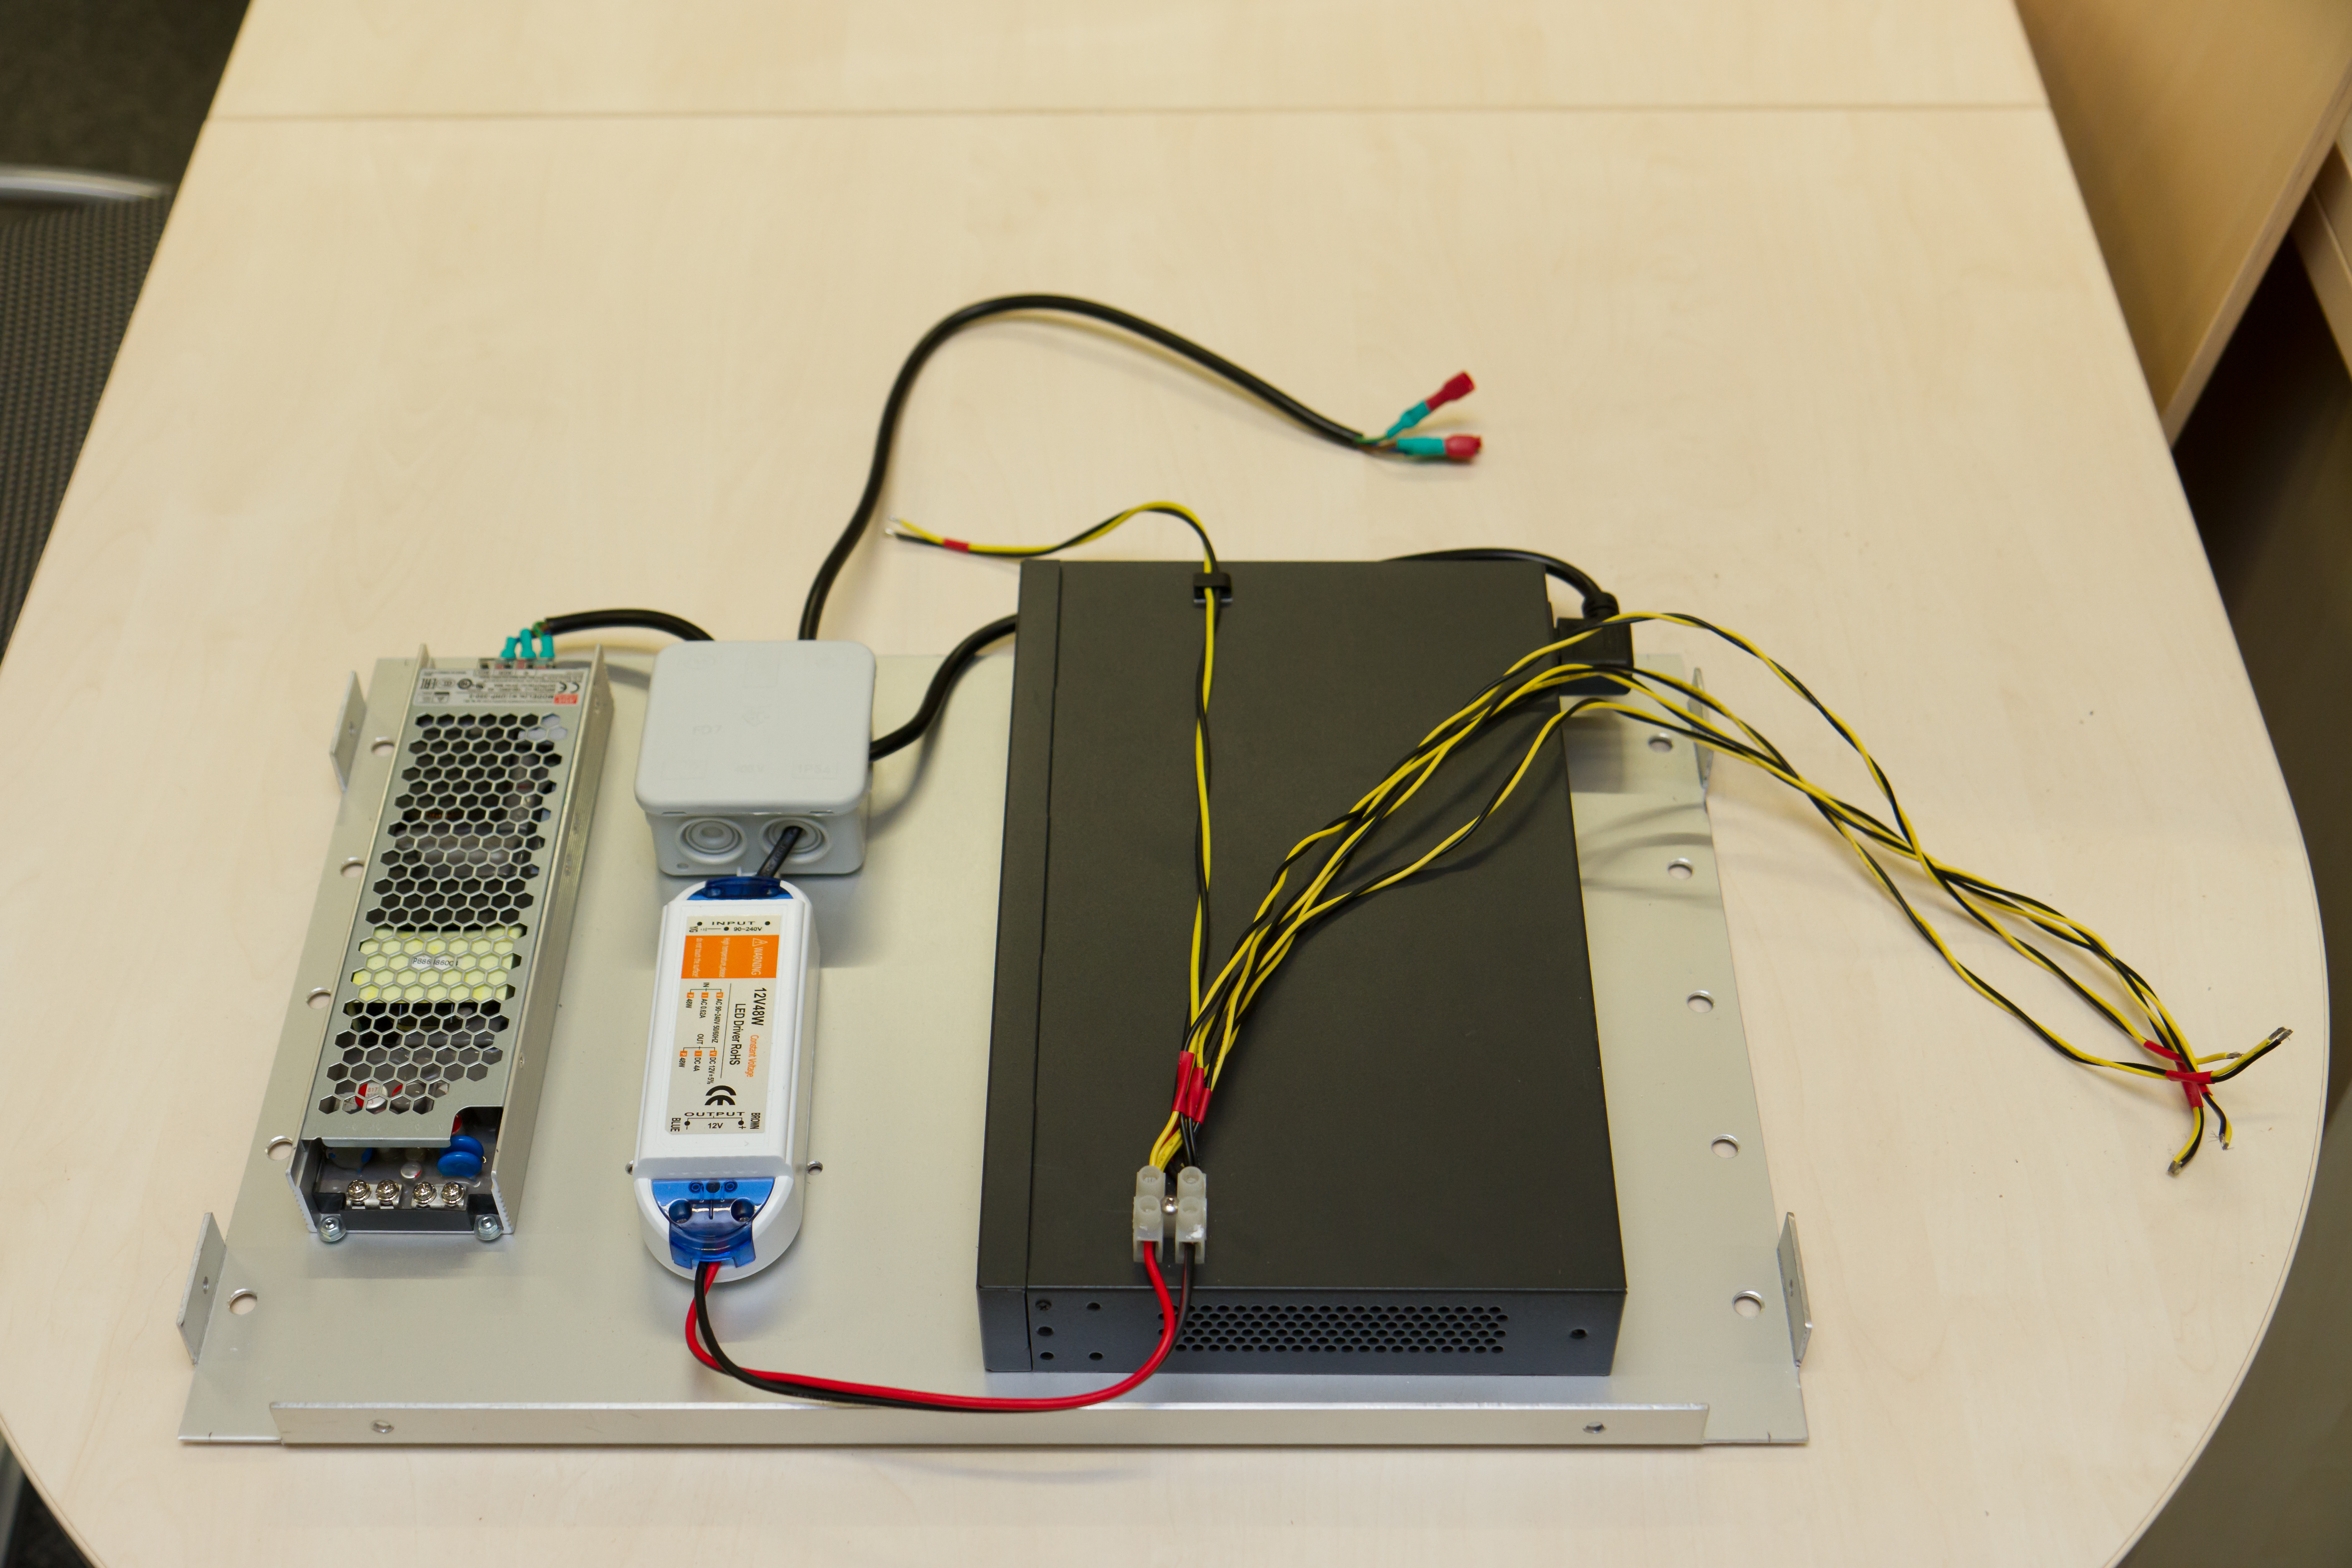
\includegraphics[width=0.95\textwidth]{inc/img_9750.jpg}
	\caption{Assembled base-plate.}
\end{figure}

\begin{figure}
	\includegraphics[width=0.95\textwidth]{inc/img_9751.jpg}
	\caption{Two assembled V-Mount panels.}
\end{figure}

\begin{figure}
	\includegraphics[width=0.95\textwidth]{inc/img_9752.jpg}
	\caption{Case backside with plug and switch.}
\end{figure}

\begin{figure}
	\includegraphics[width=0.95\textwidth]{inc/img_9753.jpg}
	\caption{Case internals with head node.}
\end{figure}

\begin{figure}
	\includegraphics[width=0.95\textwidth]{inc/img_9754.jpg}
	\caption{Assembled V-Mount panels, frame, and base-plate.}
\end{figure}

\begin{figure}
	\includegraphics[width=0.95\textwidth]{inc/img_9755.jpg}
	\caption{Fully assembled system.}
\end{figure}


\appendix
\chapter{Bill of Materials}
\label{bom}

The following table contains material required for this build.
Minor items (e.g.\ cable ties, screws) and custom made components are omitted.
Prices are approximated.

\begin{center}
\begin{longtable}{llrr}
	\toprule
	\multicolumn{2}{l}{\textbf{Item}} & \textbf{Count} & \textbf{Price (single) €}\\

	\midrule
	\multicolumn{2}{l}{Head Node}\\
	& NanoPC T4 & 1 & 95.00\\
	& Akasa AK-210 Blue Lights Northbridge Kühler & 1 & 10.00\\
	& Akasa AK-TT12-80 Wärmeleitfolie & 1 & 10.00\\
	& Micro SD Card 16GB & 1 & 4.00\\
	& Cat 7 Ethernet Cable 0.50m & 1 & 1.80\\

	\midrule
	\multicolumn{2}{l}{Compute Nodes}\\
	& NanoPI M4 2GB & 16 & 65.00\\
	& NanoPI M4 Heatsink & 16 & 5.00\\
	& Micro SD Card 16GB & 16 & 4.00\\
	& 40mm Fan (12V, 3 Pin Connector) & 16 & 6.00\\
	& Cat 7 Ethernet Cable 0.25m & 8 & 1.60\\
	& Cat 7 Ethernet Cable 0.50m & 8 & 1.80\\

	\midrule
	\multicolumn{2}{l}{Switch}\\
	& TP-Link TL-SG1024D & 1 & 70.00\\

	\midrule
	\multicolumn{2}{l}{Power}\\
	& AC Switching Power Supply 5V 300W & 1 & 60.00\\
	& AC Switching Power Supply 12V 48W & 1 & 8.00\\
	& Mains Power Socket Connector (with Switch and Fuse) & 1 & 5.00\\

	\midrule
	\multicolumn{2}{l}{Frame}\\
	& HFS5 2020 420mm (both ends tapped) & 2 & 6.00\\
	& HFS5 2020 280mm (both ends tapped) & 4 & 6.00\\
	& HFS5 2020 50mm (both ends tapped) & 4 & 6.00\\
	& HNUT5-4 M4 Nut (with spring) & 22 & 0.50\\
	& HNUT5-5 M5 Nut (with spring) & 10 & 0.50\\
	& HBLCS5-B Edge Connector 2-Way & 4 & 4.00\\
	& HBLCR5-B Edge Connector 3-Way & 4 & 4.00\\

	\midrule
	\multicolumn{2}{l}{Case}\\
	& Aluminium Suitcase (inner dimensions $486 \times 346 \times 195$ mm) & 1 & 80.00\\

	\bottomrule
\end{longtable}
\end{center}


\end{document}
